% !BIB TS-program = biber
% !BIB program = biber
\documentclass[specification,annotation,times]{itmo-student-thesis}

%% Опции пакета:
%% - specification - если есть, генерируется задание, иначе не генерируется
%% - annotation - если есть, генерируется аннотация, иначе не генерируется
%% - times - делает все шрифтом Times New Roman, собирается с помощью xelatex
%% - languages={...} - устанавливает перечень используемых языков. По умолчанию это {english,russian}.
%%                     Последний из языков определяет текст основного документа.

\usepackage{graphicx}
\graphicspath{ {./img/} }

%% Делает запятую в формулах более интеллектуальной, например:
%% $1,5x$ будет читаться как полтора икса, а не один запятая пять иксов.
%% Однако если написать $1, 5x$, то все будет как прежде.
\usepackage{icomma}

%% Один из пакетов, позволяющий делать таблицы на всю ширину текста.
\usepackage{tabularx}

%% Данные пакеты необязательны к использованию в бакалаврских/магистерских
%% Они нужны для иллюстративных целей
%% Начало
\usepackage{tikz}
\usetikzlibrary{arrows}
\usepackage{filecontents}
\begin{filecontents}{master-thesis.bib}

@online{ programmatic-buying,
    title = {Programmatic Buying - Definition and Demarcation},
    url = {https://en.ryte.com/wiki/Programmatic_Buying},
    langid = {english},
    urldate = {2020-05-26},
    year = {2020}
}

@online{ growth-of-programmatic,
    title = {How is programmatic marketing and digital display advertising defined},
    url = {https://www.smartinsights.com/internet-advertising/internet-advertising-targeting/what-is-programmatic-marketing/},
    langid = {english},
    urldate = {2020-05-26},
    year = {2020}
}

@online{ ad-server,
    title = {Ad serving},
    url = {https://en.wikipedia.org/wiki/Ad_serving},
    langid = {english},
    urldate = {2020-05-26},
    year = {2020}
}

@online{ ad-server,
    title = {Ad serving},
    url = {https://en.wikipedia.org/wiki/Ad_serving},
    langid = {english},
    urldate = {2020-05-26},
    year = {2020}
}

@online{ data-access-layer,
    title = {Data access layer},
    url = {https://en.wikipedia.org/wiki/Data_access_layer},
    langid = {english},
    urldate = {2020-05-26},
    year = {2020}
}

@online{ twelve-factor-app,
    title = {The Twelve-Factor App},
    url = {https://12factor.net/},
    langid = {english},
    urldate = {2020-05-26},
    year = {2020}
}

@online{ amazon-paapi-docs,
    title = {Product Advertising API 5.0 - documentation},
    url = {https://webservices.amazon.com/paapi5/documentation/},
    langid = {english},
    urldate = {2020-05-26},
    year = {2020}
}

@online{ amazon-paapi-sdk,
    title = {Product Advertising API 5.0 - Node.js SDK},
    url = {https://webservices.amazon.com/paapi5/documentation/assets/archives/paapi5-nodejs-sdk-example.zip},
    langid = {english},
    urldate = {2020-05-26},
    year = {2020}
}

@online{ repository-pattern,
    title = {Repository Pattern},
    url = {https://deviq.com/repository-pattern/},
    langid = {english},
    urldate = {2020-05-26},
    year = {2020}
}

@online{ contextual-targeting,
    title = {Contextual advertising},
    url = {https://en.wikipedia.org/wiki/Contextual_advertising},
    langid = {english},
    urldate = {2020-05-26},
    year = {2020}
}

@online{ behavioural-targeting,
    title = {Behavioural targeting},
    url = {https://en.wikipedia.org/wiki/Targeted_advertising#Behavioural_targeting},
    langid = {english},
    urldate = {2020-05-26},
    year = {2020}
}

@online{ creative-sequencing,
    title = {Creative sequencing},
    url = {https://en.wikipedia.org/wiki/Creative_sequencing},
    langid = {english},
    urldate = {2020-05-26},
    year = {2020}
}

@online{ capterra,
    title = {Capterra - find the best Ad Server Software for your business},
    url = {https://www.capterra.com/ad-server-software/},
    langid = {english},
    urldate = {2020-05-26},
    year = {2020}
}

@online{ revive-adserver,
    title = {Free Open Source Ad Server - Revive Adserver},
    url = {https://www.revive-adserver.net/},
    langid = {english},
    urldate = {2020-05-26},
    year = {2020}
}

@online{ google-ad-manager,
    title = {Google Ad Manager},
    url = {https://admanager.google.com/home/},
    langid = {english},
    urldate = {2020-05-26},
    year = {2020}
}

@online{ adzerk,
    title = {Build an Ad Server in Weeks | Adzerk},
    url = {https://adzerk.com/},
    langid = {english},
    urldate = {2020-05-26},
    year = {2020}
}

@online{ epom-ad-server,
    title = {Epom Ad Server | Leading Ad Serving Platform for Networks},
    url = {https://epom.com/},
    langid = {english},
    urldate = {2020-05-26},
    year = {2020}
}

@online{ mopub,
    title = {Powerful app monetization | MoPub},
    url = {https://www.mopub.com/en},
    langid = {english},
    urldate = {2020-05-26},
    year = {2020}
}

@online{ IBM-NLP,
    title = {Natural Language Understanding - IBM Cloud API Docs},
    url = {https://cloud.ibm.com/apidocs/natural-language-understanding#categories},
    langid = {english},
    urldate = {2020-05-26},
    year = {2020}
}

@online{ redis-vs-mongodb,
    title = {Redis vs. MongoDB: Comparing In-Memory Databases with Percona Memory Engine},
    url = {https://scalegrid.io/blog/comparing-in-memory-databases-redis-vs-mongodb-percona-memory-engine/},
    langid = {english},
    urldate = {2020-05-26},
    year = {2017}
}

@online{ redis-caching,
    title = {How To: Redis Caching | Redis Labs},
    url = {https://redislabs.com/redis-enterprise/use-cases/caching/},
    langid = {english},
    urldate = {2020-05-26},
    year = {2020}
}

@online{ redis-session-management,
    title = {Session Management | Redis Labs},
    url = {https://redislabs.com/redis-enterprise/use-cases/session-management/},
    langid = {english},
    urldate = {2020-05-26},
    year = {2020}
}

@online{ CAP-theorem,
    title = {CAP theorem},
    url = {https://en.wikipedia.org/wiki/CAP_theorem},
    langid = {english},
    urldate = {2020-05-26},
    year = {2020}
}

@online{ test-pyramid,
    title = {The Practical Test Pyramid},
    url = {https://martinfowler.com/articles/practical-test-pyramid.html#TheTestPyramid},
    langid = {english},
    urldate = {2020-05-26},
    year = {2018}
}

@online{ node-mongodb-native,
    title = {MongoDB Node.js Driver},
    url = {https://mongodb.github.io/node-mongodb-native/},
    langid = {english},
    urldate = {2020-05-26},
    year = {2020}
}

@online{ koa-js,
    title = {Koa - next generation web framework for node.js},
    url = {https://koajs.com/},
    langid = {english},
    urldate = {2020-05-26},
    year = {2020}
}

@online{ ioredis,
    title = {ioredis - a robust, performance-focused and full-featured Redis client for Node.js.},
    url = {https://github.com/luin/ioredis},
    langid = {english},
    urldate = {2020-05-26},
    year = {2020}
}

@online{ categories-hierarchy,
    title = {IBM Cloud Docs - Categories hierarchy},
    url = {https://cloud.ibm.com/docs/natural-language-understanding?topic=natural-language-understanding-categories-hierarchy},
    langid = {english},
    urldate = {2020-05-26},
    year = {2020}
}

@online{ JWT,
    title = {JSON Web Tokens - jwt.io},
    url = {https://jwt.io/},
    langid = {english},
    urldate = {2020-05-26},
    year = {2020}
}

@online{ OAS,
    title = {The OpenAPI Specification Repository},
    url = {https://github.com/OAI/OpenAPI-Specification},
    langid = {english},
    urldate = {2020-05-26},
    year = {2020}
}

@online{ node-clickhouse,
    title = {Yandex ClickHouse driver for nodejs},
    url = {https://github.com/apla/node-clickhouse},
    langid = {english},
    urldate = {2020-05-26},
    year = {2020}
}

@online{ gke-machine-types,
    title = {Machine types|Compute Engine Documentation|Google Cloud},
    url = {https://cloud.google.com/compute/docs/machine-types},
    langid = {english},
    urldate = {2020-06-17},
    year = {2020}
}

\end{filecontents}
%% Конец

%% Указываем файл с библиографией.
\addbibresource{master-thesis.bib}

%% Добавляем подсветку синтаксиса для ECMAScript 6
\usepackage{listings}
\usepackage{color}
\usepackage{textcomp} % for upquote

%
% ECMAScript 2015 (ES6) definition by Gary Hammock
%

\lstdefinelanguage[ECMAScript2015]{JavaScript}[]{JavaScript}{
  morekeywords=[1]{await, async, case, catch, class, const, default, do,
    enum, export, extends, finally, from, implements, import, instanceof,
    let, static, super, switch, throw, try, public, constructor},
  morestring=[b]` % Interpolation strings.
}


%
% JavaScript version 1.1 by Gary Hammock
%
% Reference:
%   B. Eich and C. Rand Mckinney, "JavaScript Language Specification
%     (Preliminary Draft)", JavaScript 1.1.  1996-11-18.  [Online]
%     http://hepunx.rl.ac.uk/~adye/jsspec11/titlepg2.htm
%

\lstdefinelanguage{JavaScript}{
  morekeywords=[1]{break, continue, delete, else, for, function, if, in,
    new, return, this, typeof, var, void, while, with},
  % Literals, primitive types, and reference types.
  morekeywords=[2]{false, null, true, boolean, number, undefined,
    Array, Boolean, Date, Math, Number, String, Object},
  % Built-ins.
  morekeywords=[3]{eval, parseInt, parseFloat, escape, unescape},
  sensitive,
  morecomment=[s]{/*}{*/},
  morecomment=[l]//,
  morecomment=[s]{/**}{*/}, % JavaDoc style comments
  morestring=[b]',
  morestring=[b]"
}[keywords, comments, strings]


\lstalias[]{ES6}[ECMAScript2015]{JavaScript}

% Requires package: color.
\definecolor{mediumgray}{rgb}{0.3, 0.4, 0.4}
\definecolor{mediumblue}{rgb}{0.0, 0.0, 0.8}
\definecolor{forestgreen}{rgb}{0.13, 0.55, 0.13}
\definecolor{darkviolet}{rgb}{0.58, 0.0, 0.83}
\definecolor{royalblue}{rgb}{0.25, 0.41, 0.88}
\definecolor{crimson}{rgb}{0.86, 0.8, 0.24}

\lstdefinestyle{JSES6Base}{
  backgroundcolor=\color{white},
  basicstyle=\ttfamily,
  breakatwhitespace=false,
  breaklines=false,
  captionpos=b,
  columns=fullflexible,
  commentstyle=\color{mediumgray}\upshape,
  emph={},
  emphstyle=\color{crimson},
  extendedchars=true,  % requires inputenc
  fontadjust=true,
  frame=single,
  identifierstyle=\color{black},
  keepspaces=true,
  keywordstyle=\color{mediumblue},
  keywordstyle={[2]\color{darkviolet}},
  keywordstyle={[3]\color{royalblue}},
  numbers=left,
  numbersep=5pt,
  numberstyle=\tiny\color{black},
  rulecolor=\color{black},
  showlines=true,
  showspaces=false,
  showstringspaces=false,
  showtabs=false,
  stringstyle=\color{forestgreen},
  tabsize=2,
  title=\lstname,
  upquote=true  % requires textcomp
}

\lstdefinestyle{JavaScript}{
  language=JavaScript,
  style=JSES6Base
}
\lstdefinestyle{ES6}{
  language=ES6,
  style=JSES6Base
}

\begin{document}

\studygroup{M42381}
\title{Разработка платформы для управления
таргетированной рекламой}
\author{Чекменев Александр Романович}{Чекменев А.Р.}
\supervisor{Фильченков Андрей Александович}{Фильченков А. А.}{к.ф.-м.н.}{доцент ФИТиП}
\publishyear{2020}
%% Дата выдачи задания. Можно не указывать, тогда надо будет заполнить от руки.
\startdate{01}{сентября}{2019}
%% Срок сдачи студентом работы. Можно не указывать, тогда надо будет заполнить от руки.
\finishdate{01}{июня}{2020}
%% Дата защиты. Можно не указывать, тогда надо будет заполнить от руки.
\defencedate{23}{июня}{2020}

%\addconsultant{Белашенков Н.Р.}{канд. физ.-мат. наук, без звания}
\addconsultant{Шевченко Е.А.}{ведущий разработчик, Fulldive corp.}

\secretary{Павлова О.Н.}

%% Задание
%%% Техническое задание и исходные данные к работе
\technicalspec{Требуется разработать рекламный сервер, обеспечивающий функционирование рекламной сети согласно установленным техническим и бизнес-требованиям.}

%%% Содержание выпускной квалификационной работы (перечень подлежащих разработке вопросов)
\plannedcontents{Описание архитектуры рекламного сервера, устройство отдельных модулей бизнес-логики, устройство хранения данных в MongoDB, Redis, ClickHouse и процесс развертывания микросервиса в кластере Google Kubernetes Engine.}

%%% Исходные материалы и пособия 
\plannedsources{нет}

%%% Цель исследования
\researchaim{Разработка рекламного сервера для функционирования тергетированной рекламной сети}

%%% Задачи, решаемые в ВКР
\researchtargets{\begin{enumerate}
\item разработка контракта клиент-серверного взаимодействия;
\item разработка архитектуры серверного приложения;
\item разработка модуля для создания и обновления рекламных объявлений на основе товаров Amazon;
\item разработка механизма получения списка объявлений с сохранением консистентности;
\item разработка алгоритмов работы стратегий таргетирования объявлений;
\item разработка системы трекинга просмотров и переходов по объявлениям с возможностью просмотра статистики по объявлениям и стратегиям таргетинга.
\end{enumerate}
}

%%% Использование современных пакетов компьютерных программ и технологий

%%% Краткая характеристика полученных результатов 
\researchsummary{Рекламная сервер запущен в production-окружении в кластере Google Kubernetes Engine. Примеры рекламных объявлений различного формата доступны в приложении Fulldive Browser на платформах iOS и Android.}

%%% Гранты, полученные при выполнении работы 
\researchfunding{нет}

%%% Наличие публикаций и выступлений на конференциях по теме выпускной работы
\researchpublications{нет}

%% Эта команда генерирует титульный лист и аннотацию.
\maketitle{Магистр}

%% Оглавление
\tableofcontents





%% Макрос для введения. Совместим со старым стилевиком.

\startprefacepage

Прогресс в сфере технологий и интеллектуальных систем неизбежно влечет за собой активное развитие всех смежных областей, а достижения вследствие такого развития внедряются и в другие сферы. Сфера digital-рекламы в этом плане не является исключением. 

Результатом применения современных подходов в digital-рекламе является, например, алгоритмическая закупка рекламы (англ. programmatic buying) \cite{programmatic-buying} — способ закупки целевого трафика с оплатой за совершенные целевые действия. Данный способ активно вытесняет традиционные способы закупки рекламы, так как обладает рядом преимуществ. Например, позволяет в режиме реального времени за долю секунды подобрать специальное рекламное объявление для каждого конкретного пользователя с учетом его демографических данных, места жительства, интересов и прочих параметров. По прогнозам маркетинговых агентств в 2020 году 69 \% digital-рекламы будет закуплено программно \cite{growth-of-programmatic}. 

Одной из причин столь активного вытеснения ранее существующих подхов стало повышение эффективности алгоритмов таргетинга. 

\begin{figure}[!h]
\caption{Рост доли алгоритмической закупки рекламы}\label{fig:share-of-programmatic}
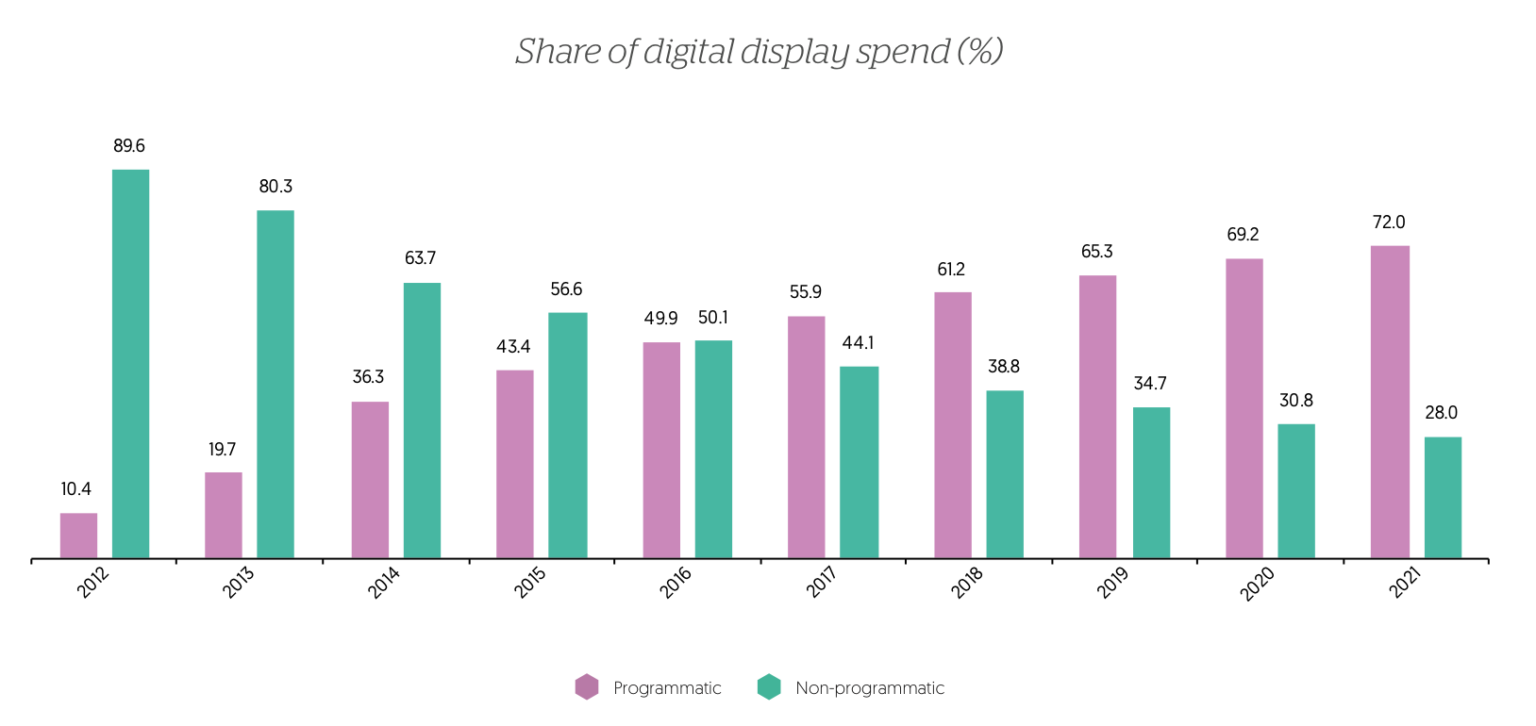
\includegraphics[width=\textwidth]{share-of-programmatic}
\centering
\end{figure}

В данный момент таргетированная реклама одна из наиболее развивающихся областей digital-рекламы, так как позволяет максимально гибко и точно задать необходимую целевую аудиторию для каждого рекламного объявления. Существует ряд компаний, предоставляющих услуги по размещению таргетированной рекламы в своих рекламных сетях. Но все они имеют такие существенные недостатки, как отсутствие прямого доступа к целевой аудитории, а также строгая зависимость от условий, устанавливаемых рекламными площадками. Все это создает трудности в воплощении нестандартных подходов для компаний, которые по каким-либо причинам не могут выполнить установленные требования, и дает все основания задуматься о создании собственной рекламной сети.

Компания Fulldive разработала приложение Fulldive VR, которое входит в топ-5 приложений для Android в категории VR. Fulldive Browser — второй активно развивающийся продукт компании. Одним из его выжнейших и эффективно влияющих на привлечение новых пользователей преимуществом является возможность пользователя монетизировать свое время, проведенное за чтением новостей, общением в социальных сетях, просмотром роликов и другими действиями, типично совершаемыми в любом другом браузере. Достигается это за счет того, что компания отдает пользователю часть прибыли, полученной от рекламных сетей за просмотры рекламы, совершенные пользователем приложении. 

Далеко не все рекламные площадки приветствуют такой способ мотивации пользователей, но реализация рекламы внутри своих приложений с использованием собственной рекламной сети поможет избежать данной проблемы. Это позволит компании в полной мере следовать своей стратегии развития, не боясь сокращения или потери доходов от рекламы в будущем, а также позволит не отдавать часть прибыли сторонним рекламным площадкам.

Таким образом, можно выделить следующие преимущества наличия у компании собственной рекламной сети:
\begin{enumerate}
	\item диверсификация риска сокращения прибыли от рекламы из-за прекращения сотрудничества с основными рекламными сетями;
	\item возможность добавлять собственные рекламные форматы;
	\item возможность более тонко настраивать где и в каком контексте будет показана реклама;
	\item возможность сбора данных непосредственного взаимодействия пользователей с рекламой (First-Party Data), которые представляют наивысшую ценность, так как является наиболее точными, качественными и принадлежат компании;
	\item возможность использовать собственную рекламную сеть для привлечения сторонних рекламодателей.
\end{enumerate}

Целью данной работы является создание собственной рекламной сети UniAds, для функционирования которой необходимо разработать рекламный сервер на основе установленных бизнес-требований.

В первой главе приводится список используемых терминов, формулируется цель и постановка решаемой задачи, рассматриваются существующие решения. В второй главе приводится архитектура предлагаемого решения поставленной задачи. В третьей главе рассматриваются аспекты, связанные с технической реализацией приведенного во второй главе решения. В заключении приводятся полученные результаты, подводятся итоги проделанной работы и предлагаются направления для дальнейшей деятельности.




%% Начало содержательной части.

\chapter{Постановка задачи и обзор существующих реализаций рекламного сервера}\label{chapter:1}

\startrelatedwork %% Так помечается начало обзора.

В начале данной главы (п. \ref{sec:terms}) приведены определения для основных терминов и понятий, используемых в работе. Затем формулируются цель работы, постановка задачи с разбиением на необходимые подзадачи и требования к результатам проделанной работы (п. \ref{sec:problem}). В конце главы проводится обзор существующих решений, удовлетворяющих сформулированным требованиям (п. \ref{sec:review}).

\section{Используемые термины и понятия} \label{sec:terms}

\subsection{Amazon \label{amazon}}

\textbf{Amazon} — это американская организация, одна из крупнейших в мире среди компаний, занимающихся продажей всевозможных товаров и услуг через сеть интернет. Также это лидер в области продаж товаром массового спроса через систему интернет-сервисов.

У Amazon есть собственная партнерская программа, в рамках которой всем парнерам начисляется от 1 до 5 \% от суммы совершенных привлеченными пользователями покупок, в зависимости от уровня партнера и категории покупаемого товара.

\subsection{Рекламная сеть}

\textbf{Рекламная сеть} (англ. ad network)\label{ad-network} — это технологическая платформа, которая обеспечивает продажи рекламных ресурсов между издателями и рекламодателями. Ключевой функцией рекламной сети является агрегация рекламного предложения от издателей и его соответствие спросу рекламодателя. Принципиальное различие между традиционными рекламными сетями в средствах массовой информации и рекламными сетями в интернете заключается в том, что рекламные сети в интернете используют рекламные серверы для таргетирования и доставки рекламы потребителям, отслеживания и составления отчетов о показах способами, невозможными при использовании аналоговых средств массовой информации.

\textbf{Таргетированная рекламная сеть} (англ. targeted ad network) — наиболее продвинутый вид рекламных сетей, которые специализируются на технологиях точного таргетирования по поведенческим или контекстным признакам и активно анализируют данные о пользователях в целях повышения стоимости инвентаря, который они продают.

\subsection{Рекламодатель}

\textbf{Рекламодатель} (англ. advertiser) — участник рекламной сети, который создает, обновляет и оплачивает рекламу продукта или услуги и, фактически, представляющий сторону спроса. 

Рекламодатель как пользователь рекламной сети:
\begin{itemize}
\item создает рекламные материалы различных форматов;
\item выбирает модель оплаты и согласно ей оплачивает приобретенные у издателя ресурсы;
\item конфигурирует целевую аудиторию для каждого управляемого им рекламного объявления;
\item управляет категориями подходящих рекламных площадок и издателей.
\end{itemize}

\subsection{Издатель}

\textbf{Издатель} (англ. publisher) — владелец рекламной площадки, на которой рекламодатель размещает свою рекламу. За данную услугу издатель взимает с рекламодателя определенную сумму в соответствии с одной из ценовых моделей размещения рекламы. Чаще всего рекламной площадкой является веб-сайт или мобильное приложение.

Издатель как пользователь рекламной сети:
\begin{itemize}
\item регистрирует рекламную площадку и указывает ее параметры: тематику, тип и объем доступной аудитории и т.д.;
\item создает элементы рекламного инвентаря, которые будут использованы для продажи рекламодателям доступные для показа рекламы места;
\item управляет категориями допустимых рекламодателей.
\end{itemize}

\subsection{Рекламный сервер} 

\textbf{Рекламный сервер} (англ. ad server) \label{ad-server} — это технологическая платформа (обычно веб-ориентированная), отвечающая за размещение, оптимизацию и распространение рекламного контента на различных веб-сайтах и в мобильных приложениях. Рекламные серверы также отвечают за управление и отслеживание рекламы, составление отчетов и выставление счетов рекламодателям.

\textbf{Показ рекламы} (англ. ad serving)\label{ad-serving} — это технологический цикл, в котором рекламный сервер используется для размещения рекламы на различных веб-сайтах и в мобильных приложениях. Механизм показа рекламы является ключевым элементом каждого рекламного сервера. Он использует сложные алгоритмы и передовые инструменты принятия решений для выбора наиболее релевантной рекламы для показа. Процесс выбора рекламы строго ограничен правилами, которые определены издателями, рекламодателями и самим рекламным сервером. Эти правила включают критерии таргетинга, частоту просмотра, место размещения рекламы, приоритет рекламы, потенциальный доход и другие параметры. 

Рекламный сервер должен учитывать все эти факторы в режиме реального времени и возвращать результат в течение миллисекунд. Любая задержка приведет к дополнительному времени ожидания загрузки страницы, что приведет к меньшему количеству просмотров страниц  и показов рекламы.

Существует два типа рекламных серверов: один — для рекламодателей, другой — для издателей (рекламных площадок). Их отличие заключается в организации данных и удобстве работы для каждой группы пользователей.

Рекламодатели используют единый сервер объявлений, где хранится рекламный контент и предоставляется функционал для отчетов по показам, кликам и другим метрикам. Такой централизованный сервис, контролирующий распространение контента на сайтах, делает удобным отслеживание и управление рекламными материалами, повышает точность таргетинга.

Издатели — владельцы площадок — имеют отдельные рекламные серверы (только для своих доменов). Это удобно, поскольку у них есть доступ только к тому рекламному контенту, который требуется для публикации, и не нужно фильтровать все рекламные материалы на централизованном сервере.

\subsection{Таргетинг}

\textbf{Таргетинг} (англ. ad targeting)\label{targeting} — рекламный механизм, позволяющий выделить из всей имеющейся аудитории только ту часть, которая удовлетворяет заданным критериям (целевую аудиторию), и показать конкретное объявление именно ей.

Цель таргетинга — создать рекламно-информационное сообщение, по своей форме и содержанию максимально ориентированное на заинтересованную в конкретном товаре/услуге часть аудитории, а также повысить эффективность взаимодействия с этой аудиторией и получить как можно большей отдачи от неё.

Преимущества таргетинга:
\begin{itemize}
\item возможность выделить ту аудиторию, заинтересованную в покупке товара или услуги;
\item возможность снизить расходы на рекламу за счёт правильного выбора таргетинга для целевой аудитории;
\item возможность разделить всю целевую аудиторию  на группы и для каждой группы сформировать уникальное предложение.
\end{itemize}

В зависимости от того, на основе какой информации принимается решение о выборе объявления, выделяют такие виды таргетинга, как контекстный и поведенческий.

\textbf{Контекстный таргетинг} (англ. contextual targeting) \cite{contextual-targeting} — это практика показа рекламы на основе содержания веб-сайта. Существует контекстный таргетинг на категории, где объявления ориентированы на страницы, которые попадают в предварительно назначенные категории, и контекстный таргетинг на ключевые слова, где объявления ориентированы на страницы, соответствующие определенным ключевым словам. 

Семантический таргетинг является наиболее эффективной формой контекстного таргетинга. Он предполагает использование машинного обучения для распознавания контекста и семантики каждой страницы, содержащей определенный контент, а не просто определение подходящих ключевых слов на странице. Когда пользователь заходит на страницу, информация о содержимом этой веб-страницы попадает на рекламный сервер, который затем сопоставляет ее с релевантными объявлениями по ключевым словам и содержанию. Чем лучше система понимает контекст страницы, тем релевантнее будет реклама.

\textbf{Поведенческий таргетинг} (англ. behavioral targeting)\label{behavioral-targeting} — это практика сегментирования клиентов на основе поведения при просмотре веб-страниц или действий в мобильном приложении. 

Данные о поведении пользователя служат для:
\begin{itemize}
\item показа релевантной, персонализированной рекламы в тот момент, когда покупатель, скорее всего, совершит покупку;
\item изучения интересов, предпочтений и планов потенциальных покупателей;
\item формирования портретов разных сегментов целевой аудитории
\item повышения лояльности к продукту и отклика на рекламу;
\item расширения целевой аудитории.
\end{itemize}

Поведенческий таргетинг позволяет показывать объявления пользователям, которые действительно заинтересованы в рекламируемом товаре или услуге. Обратиться к целевой аудитории можно даже на тех страницах, содержание которых не соответствует тематике объявления.

\subsection{Трекинг}

\textbf{Трекинг} (англ. ad tracking) \label{tracking} или отслеживание рекламы — фиксация различных событий взаимодействия пользователя с рекламой. Данными событиями, например, являются показы, клики и конверсии. Все они записываются в базу данных для дальнейшей обработки и анализа. Процесс отслеживания рекламы важен, так как помогает измерить и оценить эффективность каждого объявления.

\textbf{Конверсионная воронка}  — это последовательность совершенных на сайте пользователем действий (микроконверсий), ведущих его к конечной цели (макроконверсии), визуализированная в виде воронки, т.к. достижение каждой следующей микроконверсии в количественном выражении меньше, чем достижения предыдущей. В зависимости от того, влияют ли результаты предыдущих стадий на последующие, воронки могут быть одного из двух типов: открытые или закрытые.

Метрики — параметры, рассчитываемые на основе данных трекинга. На основе таких параметров проводится прогнозирование и анализ эффективности рекламных кампаний. 

Метрики, используемые в данной работе:
\begin{itemize}
\item OR (англ. open rate) — отношение числа показов рекламы к числу запросов рекламных объявлений;
\item CTR (англ. click-through rate) — отношение числа кликов на рекламное объявление к числу показов;
\item CPA (англ. cost per action) — отношение общей стоимости рекламы к количеству совершенных целевых действий; стоимость целевого действия.
\end{itemize}

\subsection{Клиент-серверная архитектура}

\textbf{«Клиент — сервер»} (англ. client–server) \label{client-server-model} — вычислительная или сетевая архитектура, в которой задания или сетевая нагрузка распределены между поставщиками услуг, называемыми серверами, и заказчиками услуг, называемыми клиентами. Фактически, клиент и сервер — это программное обеспечение. Обычно эти программы расположены на разных вычислительных машинах и взаимодействуют между собой через вычислительную сеть посредством сетевых протоколов, но они могут быть расположены также и на одной машине. Программы-серверы ожидают от клиентских программ запросы и предоставляют им свои ресурсы в виде данных или в виде сервисных функций.

% Сервер — это компьютерная программа или устройство, которое обеспечивает функциональность для других программ или устройств, называемых клиентами.

% Клиент — это аппаратный или программный компонент вычислительной системы, посылающий запросы серверу.

\textbf{API} \label{API} — это вычислительный интерфейс, который является контрактом взаимодействия нескольких программных комплексов. API определяет функциональность, которую предоставляет программа (модуль, библиотека), при этом API позволяет абстрагироваться от того, как именно эта функциональность реализована.

\subsection{Микросервисная архитектура}

\textbf{Микросервисная архитектура} \label{microservice-architecture} — вариант сервис-ориентированной архитектуры программного обеспечения, направленный на взаимодействие насколько это возможно небольших, слабо связанных и легко изменяемых модулей — микросервисов, получивший распространение в середине 2010-х годов в связи с развитием практик гибкой разработки и DevOps.

Свойства, характерные для микросервисной архитектуры:
\begin{itemize}
\item модули можно легко заменить в любое время: акцент на простоту, независимость развёртывания и обновления каждого из микросервисов;
\item модули организованы вокруг функций: микросервис по возможности выполняет только одну достаточно элементарную функцию;
\item модули могут быть реализованы с использованием различных языков программирования, фреймворков, связующего программного обеспечения, выполняться в различных средах контейнеризации, виртуализации, под управлением различных операционных систем на различных аппаратных платформах: приоритет отдаётся в пользу наибольшей эффективности для каждой конкретной функции, нежели стандартизации средств разработки и исполнения;
\item архитектура симметричная, а не иерархическая: зависимости между микросервисами одноранговые.
\end{itemize}

\subsection{Трехуровневая архитектура }

\textbf{Трёхуровневая архитектура} (англ. three-tier) \label{three-tier-architecture} — архитектурная модель программного комплекса, предполагающая наличие в нём трёх компонентов: клиента, сервера приложений (к которому подключено клиентское приложение) и сервера баз данных (с которым работает сервер приложений).

Клиент (слой клиента) — это интерфейсный компонент комплекса, предоставляемый конечному пользователю. Этот уровень не должен иметь прямых связей с базой данных, быть нагруженным основной бизнес-логикой и хранить состояние приложения. На этот уровень обычно выносится только простейшая бизнес-логика.

Сервер приложений (средний слой, связующий слой) располагается на втором уровне, на нём сосредоточена большая часть бизнес-логики. Серверы приложений проектируются таким образом, чтобы добавление к ним дополнительных экземпляров обеспечивало горизонтальное масштабирование производительности программного комплекса и не требовало внесения изменений в программный код приложения.

Сервер баз данных (слой данных) обеспечивает хранение данных и выносится на отдельный уровень, реализуется, как правило, средствами систем управления базами данных, подключение к этому компоненту обеспечивается только с уровня сервера приложений.

\subsection{Платформа Node.js}

\textbf{Node.js} \label{node-js}  — программная платформа, основанная на движке V8 (транслирующем JavaScript в машинный код), превращающая JavaScript из узкоспециализированного языка в язык общего назначения. Node.js добавляет возможность JavaScript взаимодействовать с устройствами ввода-вывода через свой API, подключать другие внешние библиотеки, написанные на разных языках, обеспечивая вызовы к ним из JavaScript-кода. Node.js применяется преимущественно на сервере, выполняя роль веб-сервера. В основе Node.js лежит событийно-ориентированное и асинхронное (или реактивное) программирование с неблокирующим вводом/выводом.

\textbf{NPM} (изначально сокращение от Node Package Manager ) \label{NPM} — менеджер пакетов для языка программирования JavaScript. Этот менеджер пакетов используется по умолчанию для исполняющей среды Node.js.

\subsection{TypeScript}

\textbf{TypeScript} \label{typescript}  — язык программирования, представленный компанией Microsoft в 2012 году и позиционируемый как средство разработки веб-приложений, расширяющее возможности JavaScript. TypeScript является обратно совместимым с JavaScript и компилируется в последний. Фактически, после компиляции программу на TypeScript можно выполнять в любом современном браузере или использовать совместно с серверной платформой Node.js.

\subsection{SOLID}

\textbf{SOLID} \label{SOLID} — это аббревиатура пяти основных принципов проектирования в объектно-ориентированном программировании.

Расшифровка аббревиатуры:
\begin{itemize}
\item Single responsibility — принцип единственной ответственности;
\item Open-closed — принцип открытости / закрытости;
\item Liskov substitution — принцип подстановки Барбары Лисков;
\item Interface segregation — принцип разделения интерфейса;
\item Dependency inversion — принцип инверсии зависимостей.
\end{itemize}

Эти принципы позволяют строить на базе ООП масштабируемые и сопровождаемые программные продукты с понятной бизнес-логикой.

\subsection{Базы данных}

\textbf{MongoDB} \label{mongodb} — документоориентированная система управления базами данных с открытым исходным кодом, не требующая описания схемы таблиц. Классифицирована как NoSQL, использует JSON-подобные документы и схему базы данных. Написана на языке C++. Используется в веб-разработке, в частности, в рамках JavaScript-ориентированного стека MEAN.

\textbf{Redis} \label{redis} — быстрое хранилище в памяти с открытым исходным кодом для структур данных «ключ-значение». Redis поставляется с набором разнообразных структур данных в памяти, что упрощает создание различных специальных приложений. Самые распространенные примеры использования Redis включают кэширование, управление сессиями, системы «издатель-подписчик» и таблицы лидеров. Это самое популярное на текущий момент хранилище пар «ключ-значение».

Благодаря высокой скорости и простоте Redis часто используется для мобильных и интернет-приложений, игр, рекламных платформ, «Интернета вещей», т. е. в тех случаях, когда необходима максимально возможная производительность.

\textbf{ClickHouse} \label{clickhouse} — это колоночная аналитическая СУБД с открытым кодом, позволяющая выполнять аналитические запросы в режиме реального времени на структурированных больших данных, разрабатываемая компанией Яндекс.


% \subsection{Тестирование}

% Модульное + Интеграционное + Системное


\subsection{Развертывание}

\textbf{Docker}\label{docker} — программное обеспечение для автоматизации развёртывания и управления приложениями в средах с поддержкой контейнеризации. Позволяет «упаковать» приложение со всем его окружением и зависимостями в контейнер, который может быть перенесён на любую Linux-систему с поддержкой cgroups в ядре, а также предоставляет среду по управлению контейнерами.

\textbf{Kubernetes}\label{kubernetes} — это портативная расширяемая платформа с открытым исходным кодом для управления контейнеризованными рабочими нагрузками и сервисами, которая облегчает как декларативную настройку, так и автоматизацию. У платформы есть большая, быстро растущая экосистема. Сервисы, поддержка и инструменты Kubernetes широко доступны. Поддерживает основные технологии контейнеризации, включая Docker, rkt, также возможна поддержка технологий аппаратной виртуализации.

\textbf{Google Cloud Platform} \label{GCP} — предоставляемый компанией Google набор облачных служб, которые выполняются на той же самой инфраструктуре, которую Google использует для своих продуктов, предназначенных для конечных потребителей, таких как Google Search и YouTube. Кроме инструментов для управления, также предоставляется ряд модульных облачных служб, таких как облачные вычисления, хранение данных, анализ данных, машинное обучение и многие другие.

\textbf{Google Kubernetes Engine} \label{GKE} — мощная система управления и оркестрации контейнеров Docker, выполняемых в облачной инфраструктуре Google. GKE составляет контейнеры в кластеры и управляет ими автоматически, опираясь на определенные вами требования. Google Kubernetes Engine основан на системе с открытым исходным кодом Kubernetes.




\section{Постановка задачи\label{sec:problem}}

Fulldive Browser — браузер, который, помимо втроенных возможностей социальных сетей, позволяет пользователям получать часть дохода компании от просмотренной рекламы. В приложении используется таргетированная реклама, закупаемая у сторонних рекламных сетей, таких как Google AdMob, Facebook Audience Network, MoPub, PubMatic и других. Практически каждая из приведенных рекламных сетей либо запрещает возвращать часть доходов пользователям приложения, либо накладывает существенные ограничения на объем и качество поставляемой рекламы. Подобные ограничения являются вполне обоснованным решением для создания собственной рекламной сети.

Целью данной работы является создание собственной рекламной сети UniAds, для функционирования которой необходимо разработать рекламный сервер на основе установленных бизнес-требований.

Разработка рекламного сервера (п. \ref{ad-server}) сводится к решению следующих подзадач:
\begin{itemize}
\item разработка контракта клиент-серверного взаимодействия;
\item разработка архитектуры серверного приложения;
\item разработка модуля для создания и обновления рекламных объявлений на основе товаров Amazon (п. \ref{amazon});
\item разработка механизма получения списка объявлений с сохранением консистентности;
\item разработка алгоритмов работы стратегий таргетирования объявлений;
\item разработка системы трекинга просмотров и переходов по объявлениям с возможностью просмотра статистики по объявлениям и стратегиям таргетинга.
\end{itemize}

Каждая из позадач подразумевает составление требований, разработку архитектуры необходимых модулей и их взаимодействия, программную реализацию, соответствующее тестирование полученных модулей и внедрение. 

Основными требованиями к рекламному серверу являются возможность непосредственного доступа сотрудников компании для модификации исходного кода сервера, возможность развертывания в контролируемом окружении в облачной инфраструктуре Google Cloud Platform (п. \ref{GCP}), а также желательно использование платформы Node.js (п. \ref{node-js}) при реализации сервера. Требования к каждому отдельному модулю приводятся в в описании соответствующего модуля.

\section{Обзор существующих решений\label{sec:review}}

Для применения наиболее эффективных и актуальных подходов при решении приведенных подзадач рассмотрим наиболее популярные (по рейтингу Capterra \cite{capterra}) существующие реализации функционала рекламного сервера.


Revive Adserver \cite{revive-adserver} — единственная open-source реализация на языке PHP, разработанная много лет назад в компании OpenX. Данный продукт хорошо подходит компаниям, которые:
\begin{itemize}
\item не хотят платить ежемесечную абонентскую плату за использование продукта;
\item обладают собственными инженерными ресурсами;
\item хотят существенно сэкономить ресурсы на разработку собственного решения.
\end{itemize}
И в то же время данный продукт:
\begin{itemize}
\item согласно документации не позволяет использовать собственные алгоритмы таргетинга;
\item обладает слабой гибкостью в использовании собственных рекламных форматов;
\item обладает очень скудной и местами устаревшей документаций, что затрудняет процесс интеграции данного решения в экосистему компании.
\end{itemize}


В июне 2018 года Google объявила о новом брендинге для ряда своих рекламных продуктов. Благодаря этой инициативе они объединили свой рекламный сервер DoubleClick For Publishers со своей биржей рекламы Google Ad Exchange в единую платформу под названием Google Ad Manager (GAM) \cite{google-ad-manager}. Этот инструмент призван помочь как рекламодателям, так и издателям оптимизировать процесс показа рекламы, позволяя брендам управлять рекламой и доставлять ее в различные аудитории с одной платформы. 

Данный инструмент обладает такими преимуществами, как высокая степень отказоустойчивости, тесная взаимосвязь с другими сервисами компании Google и подробная документация. Но в то же время его существенными недостатками являются:
\begin{itemize}
\item размещение на серверах компании Google без доступа к исходному коду;
\item низкий уровень гибкости форматов рекламных объявлений;
\item существенная ограниченность в применении собственных алгоритмов таргетинга;
\item пользовательские данные хранятся на серверах Google.
\end{itemize}


Adzerk \cite{adzerk} — это облачная платформа для разработки рекламных серверов. Платформа предлагает различные API для облегчения проектирования, разработки и развертывания всех видов рекламных серверов. Adzerk включает в себя несколько систем управления базами данных, таких как UserDB и ContentDB, чтобы помочь пользователям управлять ограничением частоты, поведенческим таргетингом, таргетингом на страницы, динамическим текстом объявлений и хранением информации о веб-страницах. Модуль принятия решений Adzerk предоставляет алгоритм принятия решений, который помогает пользователям управлять таргетингом кампаний и оптимизировать доходы от рекламы. 

Существенными недостатками, приводящими к невозможности использования данного сервиса компанией для достижения поставленной цели, являются:
\begin{itemize}
\item интеграция при помощи API, что не позволяет получить прямой доступ к исходному коду даже в случае размещения на собственных серверах;
\item и как следствие стандартизации программных компомент, существенно ограниченный уровень их гибкости.
\end{itemize}

EPOM Ad Server \cite{epom-ad-server} — это рекламный сервер, который обслуживает рекламные сети. Ключевыми особенностями данного сервера являются возможность создания white-label рекламной сети, широкий спектр форматов рекламных объявлений, расширенные возможности отслеживания показателей рекламных кампаний. Также имеется возможность индивидуальной разработки необходимого функционала. Платформа размещается на серверах компании EPOM, что ограничивает доступ к исходному коду для самостоятельного внесения изменений.

MoPub \cite{mopub} — платформа для монетизации мобильных приложений, принадлежащая компании Twitter. Платформа обладает всеми стандартными для рекламного сервера функциями и широко используется многими крупными компаниями. Имеются ограничения с гибкостью настройки таргетинга, а также полное отсутствие поведенческого таргетинга и таргетинга на основе содержания веб-страницы, которые на данный момент являются одними из наиболее эффективных. Также не предоставляется доступ к исходному коду платформы.

В качестве итогов проведенного обзора существующих реализаций можно привести следующие выводы:
\begin{itemize}
\item только одна из приведенных реализаций (Revive Adserver) является open-source решением c полноценным доступом к исходному коду, но использует язык программирования PHP плоохо совместимый с экосистемой микросервисов компании Fulldive;
\item максимально подходящим решением является Adzerk, которое не предоставляет доступ к исходному коду и не позволяет развернуть рекламный сервер в собственной инфраструктуре;
\item ни один из рассмотренных вариантов реализации не позволяет получать список рекламных объявлений с сохранением консистентности.
\end{itemize}

\finishrelatedwork %% Так помечается конец обзора.

\chapterconclusion

В ходе первой главы приведены определения для основных терминов и понятий, сформулированы цель, постановка задачи и подзадачи, которые необходимо решить для достижения цели. Перечислены основные требования, которым должен соответствовать рекламный сервер. Произведен обзор существующих реализаций рекламного сервера с указанием основных преимуществ и недостатков, и подведены итоги по соответствию каждого из рассмотренных решений сформулированным требованиям.





\chapter{Описание предложенного решения}\label{chapter:2}

В данной главе описываются основные компоненты рекламного сервера, клиент-серверное взаимодействие, модели данных, модули бизнес-логики и сценарии использования.

\section{Клиент-серверное взаимодействие}

Взаимодействие клиента и сервера происходит по заранее установленному контракту, реализованному поверх HTTP протокола и представляет из себя несколько сценариев. 

Основные сценарии взаимодействия:
\begin{itemize}
\item издатель запрашивает одно рекламное объявление;
\item издатель запрашивает список объявлений;
\item издатель сообщает о совершении просмотра или перехода по объявлению пользователем;
\item рекламодатель запрашивает статистику по объявлениям;
\item администратор запрашивает статистику по стратегиям таргетинга.
\end{itemize}

Совокупность приведенных сценариев взаимодействия формирует API, данные по которому передаются в формате JSON.

Разделение ответственности между клиентом и сервером происходит по модели распределенного представления данных.

\begin{figure}[h]
\caption{Разделение ответственности между клиентом и сервером}
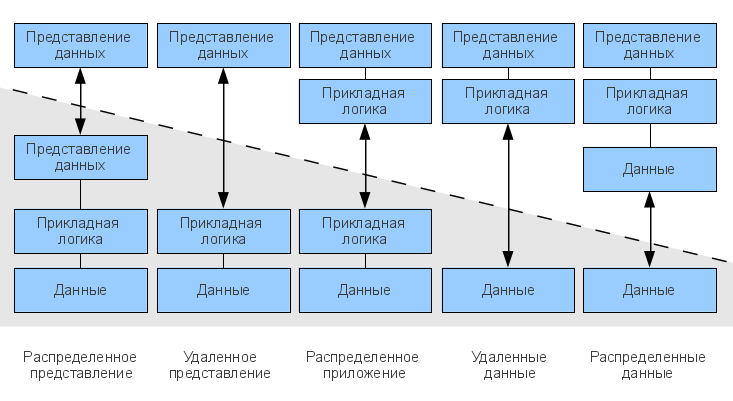
\includegraphics[width=0.75\textwidth]{cs-models}
\centering
\end{figure}

Cервер отвечает за управление рекламным инвентарем и объявлениями, сбор статистики показов, переходов и конверсий, поддержание внутренних инвариантов для сохранения актуальности и консистентности данных. Клиент отвечает за формирование запросов и корректное отображение полученных от сервера рекламных материалов и статистики.




\section{Aрхитектура серверного приложения}

  Реализацией рекламного сервера является серверное приложение. В качестве архитектуры серверного приложения используется трёхуровневая архитектура (п. \ref{three-tier-architecture}), в которой все функции разделяются на слои абстракции: слой представления, слой обработки и слой хранения данных. Разделяя приложение на слои абстракции, появляется возможность внесения изменений в отдельный слой, вместо того, чтобы перерабатывать всё приложение целиком. Трёхуровневая архитектура обычно состоит из слоя представления, слоя бизнес-логики и слоя доступа к данным.

\begin{figure}[h]
\caption{Трёхуровневая архитектура}
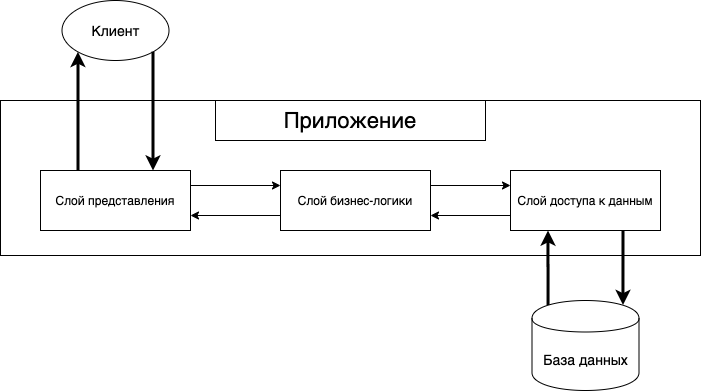
\includegraphics[width=0.75\textwidth]{three-tier-architecture}
\centering
\end{figure}



\section{Модели}\label{sec:models}

Перед тем как приступить к детальному описанию выбранной архитектуры, перечислим основные модели, которые представляют объекты предметной области, а затем последовательно рассмотрим каждый из слоев абстракции серверного приложения. 

\subsection{Модель AdProvider}

 Модель AdProvider представляет поставщика товаров, из которых впоследствии формируются рекламные объявления. Модель состоит из идентификатора провайдера, названия и ссылки на логотип для отображения ее в качестве небольшой иконки на объявлении, чтобы пользователь понимал с какой площадки представлен конкретный товар. В контексте данной работы Amazon единственный поставщик товаров.

\subsection{Модель Ad}

Модель Ad представляет рекламное объявление и состоит из следующих полей:
\begin{itemize}
\item уникальный идентификатор объявления;
\item идентификатор продукта;
\item формат объявления;
\item контент объявления, представленный ссылками на изображения и видео, используемыми для отображения объявления на клиенте;
\item ссылка для перехода на рекламируемый продукт;
\item идентификатор провайдера продукта;
\item цена продукта;
\item категория продукта.
\end{itemize}

Поддерживаемые форматы объявлений: 
\begin{itemize}
\item нативный — настраиваемый формат, соответствующий дизайну приложения;
\item баннер — платформонезависимый формат, представленный в формате HTML.
\end{itemize}

Каждый из вышепреведенных форматов также поддерживает объявления с видеоконтентом.

\subsection{Модель StrategyState \label{model:strategy-state}}

Модель StrategyState представляет состояние стратегии таргетирования и состоит из следующих полей:
\begin{itemize}
\item идентификатор стратегии (одна из стратегий, описанных в п. \ref{sec:strategies});
\item идентификтор потока (подробнее описан в п. \ref{sec:strategies-state});
\item номер версии;
\item набор пар (идентификатор объявления, скоринг объявления).
\end{itemize}

Ключ стратегии формируется из идентификатора стратегии, идентификатора потока и номера версии. Состояние стратегии предсталяет из себя набор пар идентификатор объявления и скоринг объявления, которые используются для задания порядка при запросе списка объявлений.

\subsection{Модель Session\label{model:session}}

Модель Session представляет сессию пользователя, запрашивающего рекламу из приложения. Данная модель связывает ключ сессии с ключем состояния стратегии.

\begin{figure}[h]
\caption{Связь моделей StrategyState и Session}
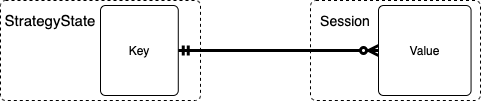
\includegraphics[width=0.75\textwidth]{strategy-state-session}
\centering
\end{figure}
Сохранение ключа состояния стратегии в сессии пользователя позволяет достичь консистентности списка объявлений при пагинации, как минимум, на время равное длительности одной сессии.

\subsection{Модели Track, Impression, Click}

Модели Track, Impression и Click необходимы для представления данных статистики рекламных объявлений. Они хранят состояние на разных стадиях жизненного цикла объявления: 
\begin{itemize}
\item запрошено клиентом — создается экземпляр Track;
\item пользователь совершил просмотр объявления — создается экземпляр Impression, связанный с уже созданным экземпляром Track;
\item пользователь совершил переход по ссылке в объявлении — создается экземпляр Click, связанный с уже созданным экземпляром Track.
\end{itemize}

Фиксирование события показа происходит на стороне клиента по истечении определенного времени (2-3 секунды), когда не менее 50 \% площади объявления видны пользователю.


\begin{figure}[h]
\caption{Связь моделей Impression, Track и Click}

\includegraphics[width=0.75\textwidth]{track-impression-click}
\centering
\end{figure}

Все три модели имеют схожую структуру полей, используемых для расчета статистики по различным срезам:
\begin{itemize}
\item идентификатор трека;
\item идентификатор рекламного объявления;
\item идентификатор элемента рекламного инвентаря;
\item идентификатор стратегии таргетинга;
\item время создания.
\end{itemize}

Модель Track также дополнительно хранит обезличенные пользовательские данные, отправляемые клиентским приложением во время запроса рекламы: тип и версия операционной системы, страна, язык, часовой пояс, версия клиентского приложения и др. Они используются в стратегиях таргетинга для увеличения вероятности клика на объявление.



\section{Слой доступа к данным}\label{sec:data-access-layer}

Слой доступа к данным (англ. data access layer) \cite{data-access-layer} взаимодействует только с вышестоящим слоем бизнес-логики и состоит из репозиториев. Репозиторий (англ. repository pattern) \cite{repository-pattern} представляет абстракцию для доступа к данным так, что приложение может работать с данными с помощью интерфейса, который приближен к интерфейсу коллекции. Каждая модель обладает собственным репозиторием.

Добавление, удаление, обновление и получение элементов из этой коллекции выполняется с помощью ряда простых методов без необходимости решать проблемы с базами данных, такие как соединения, команды, курсоры. Использование этого шаблона позволяет добиться слабой связности и отсутствия зависимости от способа хранения данных. Таким образом вся логика необходимая для функционирования моделей содержится в репозиториях.

Исходя из представленных моделей \ref{sec:models} и требований к рекламному серверу, репозитории делятся на три группы:
\begin{itemize}
\item репозиторий модели рекламного объявления ($AdRepository$, $AdMediaRepository$, $PriceRepository$);
\item репозитории моделей таргетинга ($StrategyStateRepository$, $SessionRepository$);
\item репозитории моделей трекинга ($TrackRepository$, $ImpressionRepository$, $ClickRepository$).
\end{itemize}

Также слой доступа к данным состоит из кэша рекламных объявлений (AdCache). Он необходим для сокращения времени ответа на запросы рекламы, а также для снижения количества обращений к базе данных.

\section{Слой бизнес-логики}\label{sec:business-logic-layer}

Слой бизнес-логики взаимодействует c низлежащим слоем доступа к данным и с вышестоящим слоем представления. Состоит из модулей, которые должны быть слабо связаны между собой для того, чтобы внесение изменений в один или несколько модулей не приводило к изменениям в коде всех модулей слоя.

Модуль — это высокоуровневый компонент системы, взаимодействующий с другими модулями, а также с репозиториями . При разделении бизнес-логики на модули используется подход SOLID (п. \ref{SOLID}), который обеспечивает высокую гибкость, изменяемость и поддерживаемость кода.

Далее рассмотрим каждый модуль по отедельности с указанием его назначения, алгоритма работы и диаграмм для наглядности.

\subsection{Обновление объявлений}

Обновление рекламных объявлений является автоматическим и в контексте данной работы выполняет функцию рекламодателя, т.к. генерирует объявления. 

\begin{figure}[h]
\caption{Схема процесса обновления объявлений}

\includegraphics[width=0.75\textwidth]{ad-updater}
\centering
\end{figure}
Стадии данного процеса описываются следующим алгоритмом:
\begin{enumerate}
\item отбор актуальных товаров на Amazon по заранее заданным критериям;
\item генерация рекламных объявлений на основе полученных товаров;
\item сохранение полученных объявлений в базе данных;
\item деактивация уже существующих в системе объявлений и активация только что созданных;
\item обновление объявлений в кэше.
\end{enumerate}

При обновлении объявлений в основной базе данных необходимо также обновить их и в кэше, т.к. кэш не является долгосрочным хранилищем, а лишь ускоряет доступ к актуальной версии объявлений. Выполнение обновления объявлений происходит по расписанию, установленному для соблюдения требуемого уровня актуальности.

\subsection{Обновление категорий интереса пользователя}

У каждого пользователя есть категории, которые его интересуют более остальных. Выделив подобные категории можно показывать объявления, наиболее релевантные интересам пользователя. Данный подход позволит увеличить средний CTR, что является позитивным фактором как для пользователя, который видит только интересующую его рекламу, так и для рекламодателя с издателем, которые извлекают дополнительную прибыль.
 
 Выделение категорий интереса пользователя происходит на основе анализа посещенных веб-страниц. Каждой странице на основе алгоритмов машинного обучения сопоставляется список категорий, наиболее релевантных данной странице. Для каждого пользователя хранится вектор пар категорий и соответствующее количество посещений веб-страниц по данной категории за 30 дней. Схожим образом для каждого пользователя подсчитывается еще один вектор пар категорий рекламных объявлений и количество переходов по объявлениям данной категории за 30 дней.
 
Отсортировав каждый из двух полученных векторов по невозрастанию количества посещений/переходов  и выбрав первые 5 категорий в каждом, получим два профиля краткосрочных интересов пользователя, которые теперь можно использовать в таргетинге.

\subsection{Таргетинг}

Ранжирование — механизм подбора рекламного объявления для показа пользователю таким образом, чтобы вероятность перехода по нему была наиболее высокой.

До тех пор пока данные о совершенных пользователями покупках недостпуны, ранжирование производится по показателю CTR вместо более эффективного CPA.

\begin{figure}[h]
\caption{Схема процесса таргетинга}
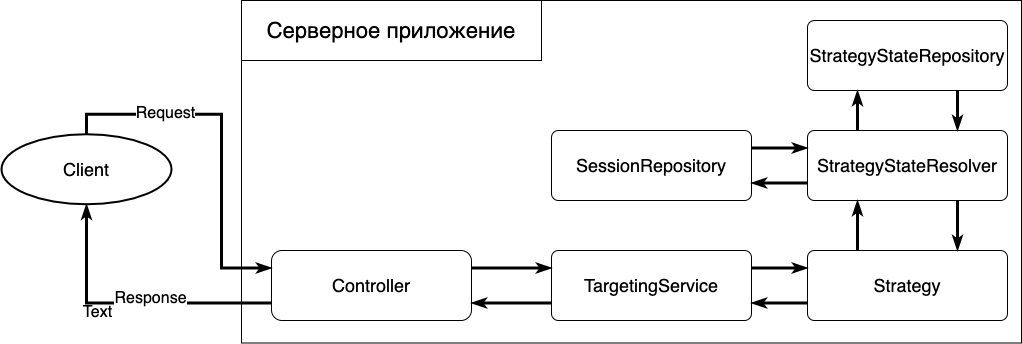
\includegraphics[width=0.75\textwidth]{targeting-process}
\centering
\end{figure}

В рамках данной работы алгоритм таргетинга состоит из следующих этапов:
\begin{itemize}
\item фильтрация всех доступных объявлений на основе параметров запроса и профиля пользователя;
\item выбор для каждого товара одного объявления с наивысшим CTR;
% \item определение каждого объявления в одну из трех групп testing, rejected, approved на основе числе показов и CTR
% \item ранжирование по группам в порядке approved, testing, rejected
% \item ранжирование внутри группы по CTR
\item ранжирование объявлений по невозрастанию CTR;
\item получение одного или нескольких объявлений из итогового списка.
\end{itemize}

Стратегия таргетинга — реализация вышепреведенного алгоритма с применением конкретных подходов для фильтрации, ранжирования и выбора рекламных объявлений. Для каждой стратегии формируется свой набор отранжированных списков объявлений (состояний стратегии) и сохраняется в кэш (репозиторий состояний стратегии), чтобы ускорить процесс получения объявлений. Выбор того или иного списка при запросе объявлений определяется логикой стратегии, а также параметрами пользователя, запрашивающего объявления. 

Каждая стратегия таргетирования назначает веса рекламным объявлениям \cite{creative-sequencing}, чтобы управлять их частотой показа. Рандомизация применяется для равномерного выбора объявлений. 
% Три группы объявлений (нарисовать автомат переходов): testing, rejected, approved.

Выбор оптимальной стратегии на основе данных, представленных в запросе. Если рекламное объявление должно зависеть от контекста, в котором оно будет показано, выбирается одна из стратегий, которая таргетирует на основании параметров переданного контекста. Иначе выбирается стратегия, которая таргетирует на основании накопленных данных о категориях интереса текущего пользователя.

\subsection{Состояния стратегий}\label{sec:strategies-state}

Ранее было преведено определение понятию "состояние стратегии" (п. \ref{model:strategy-state}). Далее будет рассмотрена концепция разделения состояний стратегий на "потоки".

Поток (англ. thread) — совокупность состояний стратегии, объединенных общим признаком (фильтром) и отсортированных в хронологическом порядке. Иными словами, поток представляет последовательность слепков (англ. snapshot) ранжирований объявлений, объединенных общим признаком. Идентификатор потока является строкой. Такой подход является компромиссом между ресурсоемким ранжированием объявлений при каждом запросе объявлений и устареванием показателей каждого объявления, зависящих от количества просмотров и кликов. 

Каждое новое ранжирование обяъвлений для конкретного потока, становится состоянием стратегии последней версии и обновляет индекс последней версии данного потока для того, чтобы быстро получать доступ к последней версии в кэше. Каждое состояние получает адрес в кэше (ключ состояния стратегии) согласно идентификатору стратегии, потоку и номеру версии состояния. По этому адресу состояние сохраняется и запрашивается. Состояние не может быть изменено.

% обновление состояний потока по расписанию

% (тут картинка потоков)

Основной поток ($general$) каждой стратегии содержит в себе все возможные объявления, доступные для данной стратегии. Также существуют потоки для категорий объявлений и для пользователей. Они позволяют ранжировать объявления в рамках одной категории или ранжировать только те объявления, которые потенциально будут интересны конкретно взятому пользователю. Это позволяет избегать показов объявлений неинтересных пользователям.

При запросе рекламных объявлений используется существующая или создается новая сессия. Как уже упоминалось ранее (п. \ref{model:session}), сессия хранит в себе ключ состояния стратегии для доступа к одному и тому же состоянию стратегии при запросах в рамках одной сессии, что позволяет сохранить консистентность при пагинации списка объявлений. Связь сессии с состоянием стратегии реализована при помощи структурного шаблона проектирование $Flyweight$ для уменьшения потребления оперативной памяти при хранении большого количества сессий. За сопоставление состояния стратегии каждой новой сессии отвечает компонент $StrategyStateResolver$. 

% (тут листинг с методом resolve)

\subsection{Стратегии таргетинга}\label{sec:strategies}

В данной работе рассматриваются 4 стратегии таргетинга объявлений.
Каждая из рассматриваемых далее стратегий гарантирует:
\begin{itemize}
\item распределение частот показа объявлений пропорционально распределению их CTR;
\item консистентность при запросе списка объявлений с пагинацией в рамках одной сессии.
\end{itemize}

Для выполенения этих требования у каждой стратегии (наследники класса StatefulStrategy) имеются:
\begin{itemize}
\item метод $getState(stateKey, offset, limit)$ — для получения из состояния с ключем $stateKey$ списка объявлений длины limit, начиная с позиции offset;
\item метод $updateState()$ — для генерации нового списка отранжированных объявлений.
\end{itemize}
Реализации стратегии по сути сводится к реализации этих двух методов.

% \textbf{Требования к показу единичных объявлений:}
% \begin{itemize}
% 	\item возможность задания категории объявления
% 	\item возможность задания списка стран, в которых будет показано объявление
% 	\item консистентность списка для пользователя / конкретного девайса пользователя
% 	\item возможность фильтрации провайдеров / товаров?
% 	\item возможность учета для каждого товара из списка: показов и кликов
% \end{itemize}

Стратегия, возвращающая случайные объявления, разработана первой по счету и использована для ускоренного запуска первой версии рекламного сервера. Логика данной стратегии тривиальна: метод $updateState$ генерирует новое состояние стратегии в основном потоке с ранжированием в случайном порядке, которое затем используется методом $getState$.

Стратегия, возвращающая отранжированные по CTR объявления, описывается следующим образом:
\begin{itemize}
\item в данной стратегии используется только основной поток;
\item метод $updateState$ генерирует новое состояние стратегии в основном потоке с ранжированием всех объявлений по невозрастанию CTR.
\end{itemize}

Последующие две стратегии используют множество потоков: для каждой категории объявлений свой поток. Обе эти стратегии возвращают отранжированные по CTR объявления в рамках заданной категории и описываются следующим образом:
\begin{itemize}
\item у объявлений каждой категории свой отдельный поток, содержащий состояния стратегии, рассчитанные только на основе объявлений данной категории;
\item метод $updateState$ генерирует новое состояние стратегии для каждой категории в соответствующем потоке с ранжированием объявлений данной категории по невозврастанию CTR;
\item  ключ состояния стратегии, передаваемый в метод $getState$, формируется на основе случайного выбора одной из пяти категорий интереса пользователя.
\end{itemize}

Отличаются они лишь методом определения категорий интереса пользователя. В одной из стратегий категории интереса пользователя определяются на основе просмотренных веб-страниц при помощи сервиса IBM Watson Natural Language Understanding \cite{IBM-NLP}:
\begin{itemize}
\item каждые 24 часа агрегируется список посещенных пользователем веб-страниц, заданных с помощью URL;
\item на основе каждого URL из списка формируется запрос к IBM Watson API;
\item из ответа на каждый запрос извлекается список категорий, отсортированных по невозрастанию релевантности данной веб-странице;
\item каждая категория из списка сопоставляется категории товаров на Amazon;
\item для каждой полученной категории увеличивается соответствующий счетчик числа посещений пользователем веб-страниц этой категории;
\item счетчики числа посещений категории хранят данные за последние 30 дней.
\end{itemize}

В второй стратегии категории интереса пользователя определяются на основе переходов по рекламным объявлениям:
\begin{itemize}
\item каждые 24 часа агрегируется список посещенных пользователем рекламных объявлений;
\item каждое объявление имеет единственную категорию, соответствующую категории товара;
\item увеличивается счетчик числа посещений пользователем товаров данной категории;
\item счетчики числа посещений категории хранят данные за последние 30 дней.
\end{itemize}

\subsection{Трекинг показов и переходов}

Трекинг показов и переходов сводится к фиксации изменений стадий жизненного цикла показа объявления пользователю. Жизненный цикл показа объявления состоит из следующих стадий:
\begin{itemize}
\item запрос объявления для показа — событие Track фиксируется сервером;
\item объявление просмотрено пользователем — событие Impression фиксируется клиентом и отправляется на сервер;
\item пользователь совершил переход по объявлению — событие Click фиксируется сервером в момент перехода с помощью редиректа.
\end{itemize}

Последовательные изменения стадий жизненного цикла, формируют закрытую конверсионную воронку (п. \ref{tracking}). 

Подобные воронки используются для анализа эффективности рекламных объявлений. По данным стадиям воронки можно выделить следующие показатели эффективности: 
\begin{itemize}
\item Open rate (OR) — отношение числа событий Impression к числу событий Track;
\item Click-through rate (CTR) — отношение числа событий Click к числу событий Impression.
\end{itemize}

\begin{figure}[h]
\caption{Закрытая конверсионная воронка}
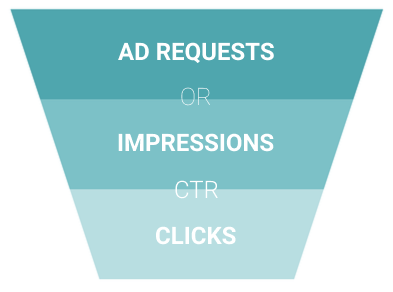
\includegraphics[width=0.5\textwidth]{funnel}
\centering
\end{figure}

Данные показатели рассчитываются как в статистике рекламных объявлений для учета при ранжировании в статегиях таргетинга, так и в статистике стратегий таргетинга для оценки эффективности работы стратегии.

% \begin{itemize}
% 	\item расчет статистики по рекламным объявлениям: Impressions, Clicks, Conversions, CTR, CR для отображение в панели рекламодателя
% 	\item оптимизация бизнес-процесса на основе данных (Data-driven decision making)
% 	\item автоматический выбор стратегии таргетирования на основе статистики стратегий
% \item возможность просмотра статистики каждого рекламного объявления в формате (AdId, Показы, Клики, CTR, тут колонки таблицы) с фильтрацией по … и группировкой по …
% 	\item возможность просмотра параметров эффективности (OR, CTR) стратегий таргетинга, рассчитанных по данным трекинга, с фильтрацией по интервалу дат и группировкой по идентификатору стратегии
% \end{itemize}

% \section{Сценарии использования}

% Сценарии использования подробно описывают использование клиентом API, предоставляемого сервером. Далее перечисляются основные сценарии взаимодействия  с указанием параметров запроса, формируемых клиентом, и логики соответствующего контроллера, обрабатывающего запрос на стороне сервера.

% Слой клиента представляет из себя контракт взаимодействия клиента и сервера. Получение данных клиентом подразумевает отправку HTTP запросов  на сервер в установленном формате и с токеном для подтверждения доступа. Среди всех сценариев можно выделить два типа триггеров: запрос к серверу, запуск по расписанию в контексте задачи.

% Далее рассмотрим совместное функционирование приведенных модулей в основных сценариях использования.

% \subsection{Получение одного объявления}

% Получение данных пользователя. 
% Выбор стратегии таргетинга. 
% Получение списка объявлений по выбранной стратегии.

% \subsection{Получение списка объявлений}

% Получение данных пользователя и текущей сессии (у каждой сессии свой уникальный ключ). 
% Выбор стратегии таргетинга. 
% Получение списка объявлений по выбранной стратегии.

% \subsection{Трекинг показов и переходов}

% TODO

% \subsection{Получение статистики по стратегиям таргетинга}

% TODO

\chapterconclusion

В ходе второй главы рассмотрен формат клиент-серверного взаимодействия, приведена архитектура серверного приложения, перечислены основные модели и компоненты бизнес-логики, а также описан процесс их работы. Рассмотрен алгоритм таргетинга объявлений и 4 его реализации в виде стратегий таргетинга с описанием хранения и обновления их состояний. В заключении описан процесс трекинга событий для расчета статистики рекламных объявлений и статистики стратегий таргетинга.



\chapter{Техническая реализация и внедрение предложенной архитектуры}

В данной главе подробно рассматриваются детали технической реализации рекламного сервера, а также описание необходимых для её осуществления процессов разработки, тестирования и развертывания.

Текущая инфраструктура компании представлена несколькими Kubernetes (п. \ref{kubernetes}) кластерами (по одному на каждое окружение). Серверные приложения являются микросервисами (п. \ref{microservice-architecture}), которые развертываются в кластере и общаются между собой по протоколу AMQP. Разделение всей серверной бизнес-логики на микросервисы производится по функциональному принципу. 

Для реализации рекламного сервера также выбрана микросервисная архитектура, которая позволяет обеспечить автономность, хорошую масштабируемость и слабую связность компонент рекламного сервера с компонентами других микросервисов.

В качестве программной платформы, исполняющей исходный код сервера, выбрана платформа Node.js (п. \ref{node-js}). Она предоставляет необходимый функционал для реализации стандартных возможностей веб-сервера,  для взаимодействия с устройствами ввода-вывода (работа с файловой системой, сетевые запросы), для подключения сторонних модулей с помощью NPM (п. \ref{NPM}) и многое другое. Это позволяет реализовать большую часть функционала посредством стандартных или сторонних модулей. 

В качестве основного языка программирования используется TypeScript (п. \ref{typescript}). Основные преимущества данного языка:
\begin{itemize}
\item широко используется в различных проектах компании, что уменьшает порог вхождения членов команды;
\item современный язык, разработанный и поддерживаемый компанией Microsoft — гарантия надежности и развития языка;
\item предоставляет возможность написания кода как в императивном стиле, так и декларативном, что позволяет повысить читаемость кода и сократить его объем за счет использования подходов из функционального программирования;
\item обладает строгой типизацией — существенное сокращение вероятности появления дефектов в процессе разработки и сопровождения кода.
\end{itemize}

Весь исходный код серверного приложения представляется в виде пакета NPM. Основные параметры пакета (название, версия, ссылка на репозиторий и прочие), скрипты и подключенные сторонние модули подробно описываются в конфигурационном файле пакета — $package.json$. Скрипты представляют из себя команды для проверки синтаксиса, сборки, тестирования и запуска приложения.

В качестве решения для контейнеризации среды исполнения кода приложения используется Docker. Расположенный в корневой директории проекта файл Dockerfile описывает процесс создания образа, который впоследствии будет отправлен в облачный реестр образов и использован для развертывания микросервиса в Kubernetes кластере.

Развернутый в кластере микросервис взаимодействует с другими микросервисами, обмениваясь сообщениями по протоколу AMQP, и предоставляет API (п. \ref{API}) для получения внешних запросов по протоколу HTTP. Для обработки поступающих запросов используется Node.js фреймворк Koa \cite{koa-js}.

В качестве DNS серверов используется сервис Cloudflare, который также фильтрует подозрительный трафик и кеширует статические файлы такие как, например, изображения и видео, используемые в рекламе.

В следующих параграфах более детально описывается устройство моделей БД, детали реализации отдельных модулей бизнес-логики, устройство методов API и алгоритм развертывания в Kubernetes кластере.




\section{Работа с моделями}

Каждая модель представлена в базе данных одной или несколькими сущностями в зависимости от сложности структуры модели. Каждой сущности соответствует репозиторий, предоставляющий методы для их создания, получения, изменения и удаления из БД. Далее подробно рассматриваются модели и соответствующие им сущности.

\subsection{Модели рекламного объявления}

Для хранения товаров, полученных с помощью Amazon Product Advertising API, используется сущность $AmazonItem$. Модель $Ad$ представляет рекламное объявление и состоит из 3 сущностей: $Ad$, $AdMedia, $  $Price$. Модель разделяется на сущности для удобства представления отношений "один-к-одному" и "один-ко-многим": 
\begin{itemize}
\item одной сущности $AmazonItem$ соответствует одна сущность Price;
\item одной сущности $Price$ соответствует много сущностей $Ad$;
\item одной сущности $Ad$ соответствует много сущностей $AdMedia$.
\end{itemize}

% (диаграмма классов с указанием отношений one-to-many)

Для хранения вышеперечесиленных сущностей используется NoSQL база данных MongoDB (п. \ref{mongodb}). Выбор произведен в пользу данной базы, поскольку:
\begin{itemize}
\item MongoDB — масштабируемая база данных общего назначения;
\item хорошо сочетается с экосистемой Node.js;
\item в терминах теоремы CAP \cite{CAP-theorem} обеспечивает строгую консистентность данных и позволяет разделять их на шарды;
\item позволяет достаточно быстро и просто расширять схему данных без миграции всех данных в коллекции;
\item является основной БД компании.
\end{itemize}

Каждая сущность имеет собственный репозиторий, который реализует функционал создания, получения, изменения и удаления сущностей в соответствующей коллекции MongoDB. Перечисленный функционал репозиториев реализуется при помощи стандартного MongoDB драйвера для Node.js \cite{node-mongodb-native}. 

\subsection{Модели таргетинга}

Для обеспечения работы таргетинга необходимы модели: 
\begin{itemize}
\item $Session$  — для хранения состояния сессии пользователя;
\item $StrategyState$ — для хранения состояния стратегии.
\end{itemize}

% (диаграммы классов данных моделей)

% Добавить эти модели и репозитории для них во вторую главу

Также для каждого пользователя хранятся такие модели, как
\begin{itemize}
\item $PageViewsProfile$ — вектор количества посещений сайтов каждой из 316 категорий второго уровня \cite{categories-hierarchy};
\item $AdClicksProfile$ — вектор количества кликов по товарам каждой из 50 допустимых категорий товаров Amazon (Приложение \ref{sec:app:categories}).
\end{itemize}
Оба профиля также содержат поля $userId$ для связи профиля с пользователем и $createdAt$  — время создания профиля.

% (диаграммы классов данных моделей)

Исходя из частоты и характера сценариев использования этих моделей (частые чтения, редкие записи), необходима максимальная скорость получения их из БД. Для решения такой задачи идеально подходит база данных Redis (п. \ref{redis}), поскольку:
\begin{itemize}
\item Redis — это нереляционная высокопроизводительная СУБД;
\item подходит для управлением состояний сессий \cite{redis-session-management};
\item позволяет эффективно кэшировать данные \cite{redis-caching};
\item в случае существенного преобладания количества чтений данных над количеством записей показывает себя более эффективным инструментом, чем MongoDB \cite{redis-vs-mongodb}.
\end{itemize}

Каждая сущность имеет собственный репозиторий, который реализует функционал создания, получения, этих моделей. Данный функционал репозиториев реализуется при помощи модуля $ioredis$ \cite{ioredis}.

\subsection{Модели трекинга и счетчиков категорий}

В трекинге участвуют такие модели, как $Track$, $Impression$, $Click$. Они соответствуют событиям, фиксируемым в процессе показа рекламных объявлений.

% (диаграммы классов данных моделей)

Указанные модели являются ключевыми данными, на основе которых рассчитывается статистика рекламных объявлений и стратегий таргетинга, по которым производится анализ эффективности объявлений и рекламного сервера в целом. Примером подобной технологии является OLAP (онлайн обработка аналитических запросов) — технология обработки данных, заключающаяся в подготовке суммарной (агрегированной) информации на основе больших массивов данных, структурированных по многомерному принципу.

В качестве хранилища для вышеперечисленных моделей выбрана база данных ClickHouse (п. \ref{clickhouse}), поскольку:
\begin{itemize}
\item ClickHouse — СУБД для OLAP;
\item ClickHouse является колоночной базой данных, которая отлично подходит для хранения структур представленных векторами: векторы категорий веб-страниц и товаров, профили пользователей.
\end{itemize}

Счетчики категорий представлены векторами состоящими из 0 и 1. Для категорий веб-страниц вектор имеет размерность 316, для категорий товаров — 50. Вектора каждого из двух типов хранятся в соответствующих таблицах семейства MergeTree базы данных ClickHouse.

Для создания и получения этих моделей в БД также используются репозитории на основе драйвера для Node.js \cite{node-clickhouse}.  Каждому элементу вектора соответствует собственная колонка в таблице базы данных.




\section{Обновление объявлений}

Класс $AdUpdater$ отвечает за периодическое автоматическое обновление рекламных объявлений. Обновление объявлений описывается следующим алгоритмом:
\begin{itemize}
\item получить товары Amazon согласно установленным параметрам фильтрации: товар доступен для приобретения в США, наличие скидки, категория товара входит в список допустимых (Приложение \ref{sec:app:categories});
\item генерация рекламных объявлений на основе полученных товаров Amazon;
\item обновление списка активных рекламных объявлений;
\item обновление рекламных объявлений в кэше.
\end{itemize}

\subsection{Получение товаров Amazon}

На данный момент официальным способом доступа к товарам, размещаемым на площадке Amazon является интерфейс Product Advertising API 5.0 \cite{amazon-paapi-docs}. Доступ к API осуществляется с помощью $access\-token$, который выдается после успешного прохождения авторизации на площадке. Взаимодействие происходит по HTTP протоколу, формат запросов и ответов — JSON. Для осуществеления авторизованных запросов используется Node.js SDK \cite{amazon-paapi-sdk}.

В ссылку на товар подставляется $PartnerTag$ для связывания покупок, совершаемых по данной ссылке, с партнером, который привел покупателя.

% (Пример ссылки)

\subsection{Создание объявления}

Класс $AdService$ отвечает за получение и обновление текущих объявлений и деактивацию неактуальных. $AdService$ имеет в качестве зависимостей репозитории $AdRepository$, $AdMediaRepository$, $PriceRepository$ для ощуствления операций над внутренними сущностями модели $Ad$.

% (диаграмма класса AdService)

Класс $AdUpdater$ на основе полученного списка товаров с Amazon генерирует список моделей $Ad$, которые затем передаются в метод $update$  класса $AdService$. Данный метод в свою очередь разделяет экземпляр модели Ad на сущности $Ad$, $AdMedia$, $Price$ и передает их в методы репозиториев, которые создают или обновляют сущности в MongoDB.

При создании нового объявления все связанные с ним медиаресурсы сохраняются в Google Bucket, который также предоставляет функции CDN. Медиаресурсы уникализируются по ссылке для того, чтобы не создавать копии уже сущетвующих файлов в Google Bucket. 

При создании или обновлении объявлений необходимо также обновить их данные и в кэше. За это отвечает класс $AdCache$, который использует Redis для кэша и стандартный модуль $class\-transformer$  для автоматической сериализации и десериализации модели Ad.




\section{Обновление категорий интереса пользователя}

Каждому просмотру веб-страницы пользователем сопоставляется вектор размера 316 (количество категорий веб-страниц), состоящий из 0 и 1, где 1 на позиции категории означает, что веб-страницу можно отнести к этой категории, 0 — иначе. Список категорий, соответствующих веб-странице, получается путем HTTP запроса к IBM Watson Natural Language Understanding API. Список категорий, полученный в результате запроса, трансформируется в вектор по вышеупомянутому правилу.

% (Пример ответа от IBM Watson NLU API (запрос по url + список категорий в ответе)

Аналогичным образом каждому клику по рекламному объявлению сопоставляется вектор длины 50 (количество категорий товаров), состоящий из 0 и 1, где 1 на позиции категории означает, что товар относится к этой категории, в противном случае — 0.

Запускаемый раз в сутки модуль $ProfileUpdater$ для каждого пользователя рассчитывает 2 профиля:
\begin{itemize}
\item $PageViewsProfile$ — на основе векторов категорий веб-страниц, посещенных за последние 30 дней;
\item $AdClicksProfile$ — на основе векторов категорий товаров Amazon, просмотренных за последние 30 дней.
\end{itemize}
Оба профиля рассчитываются группировкой векторов по $userId$, которая производится посредством базы данных ClickHouse. Колонки категорий при группировке суммируются.

% (Примеры полученных векторов счетчиков категорий)

Рассчитанные профили в формате JSON сохраняются в $hash$ Redis.  Они используются в соответствующих стратегиях таргетинга для выбора состояний стратегий, которые содержат наиболее релевантные текущим интересам пользователя объявления. Новые профили замещают имеющиеся в Redis при сохранении.




\section{Обновление состояний стратегий }

Для обновления состояний стратегий существует класс $StrategyStateUpdater$. Он запускается раз в сутки по расписанию и вызывает метод $updateState$ каждой из 4-х стратегий таргетинга. Вызов данного метода генериует новое состояние стратегии для каждого потока, который она использует. Как уже упоминалось ранее, состояние стратегии содержит в себе отранжированный список некоторого подмножества рекламных объявлений, объединенных общим признаком (категория товара, релевантность для пользователя). 

Метод $updateState$ использует репозиторий $StrategyStateRepository$ для сохранения нового состояния в Redis. Время жизни каждого состояния — 1 сутки, после истечения данного срока Redis автоматически их удаляет. Периодическое сохранение актуального состояния с одной стороны позволяет поддерживать актуальность ранжирования объявлений, а с другой стороны избавляет от неоправданного использования серверных ресурсов, в случае если бы ранжирование производилось при каждом запросе.

Детали реализации метода $updateState$ зависят от логики конкретной стратегии. Стратегия, ранжирующая объявления на основе CTR, при обновлении своего состояния раз в 15 минут запрашивает актуальную статистику объявлений с помощью класса $TrackService$. Стратегии, учитывающие при ранжировании категории интереса пользователей, получают профиль категорий интереса при помощи класса $ProfileService$.

Метод $getAdStats$ класса $TrackService$ производит группировку просмотров и кликов по $adId$ для всех активных объявлений. Результат вызова данного метода используется при обновлении состояния стратегии, ранжирующей по CTR. 

% Обновление состояния стратегии, использующей вектор категорий интереса пользователя, рассчитанный на основе истории просмотров веб-страниц ...
% Пример маппинга из категории IBM в Amazon.

% Вставки с кодом для иллюстрации  StrategyState.updateState(…) на примере 1–2 стратегий




\section{Методы API}

Контроллеры, соответствующие методам API,  спроектированы так, чтобы содержать минимальное количество бизнес-логики. Такой подход обеспечивает слабую связность контроллеров и бизнес-логики, что упрощает процесс их тестирования.

В контексте платформы Node.js процесс обработки запросов является примером поведенческого шаблона проектирования Chain of Responsibility. Для каждого запроса последовательно выполняются все обработчики цепи (middlewares). Реализация метода API сводится к созданию обработчика и помещению его в цепочку вывозов, соответствующую этому методу API.

Для аутентификации запросов к API и передачи данных сессии используется стандарт JSON Web Token (JWT) \cite{JWT}. Для автоматической генерации документации методов API используется OpenAPI Specification (OAS) \cite{OAS} — спецификация, определяющая стандартное, независимое от языка программирования описание для API. Файл openapi.yml, расположенный в корне проекта, содержит описание методов API согласно данной спецификации. Для доступа к сгенерированной документации неоьходимо сделать HTTP запрос $GET /doc$.

\subsection{Методы для получения объявлений}

% Список контроллеров, по каждому входные параметры и выходные параметры (объемные ответы в виде ссылок на примечание)

Класс $TargetingService$ предназначен для получения объявлений с наиболее высокой вероятностью перехода по ним. В зависимости от параметров пользователя и контекста запроса выбирается наиболее подходящая стратегия таргетинга. Класс имеет метод $getNextAd$ для получения одного объявления, и метод $getAdsRange$ для получения части списка длины $limit$, начиная с позиции $offset$.

% Вставки с кодом для иллюстрации StrategyStateResolver.resolve(…)

Для получения рекламных объявлений в API предусмотрено 2 метода:
\begin{itemize}
\item $POST /get\_ad $ —  вызывает метод $getNextAd$ с параметрами запроса (страна, язык, операционная система, идентификатор пользователя, ключ сессии и пр.), возвращает одно объявление;
\item $POST /get\_ads $  — вызывает метод $getAdsRange$ с параметрами запроса, возвращает список объявлений с пагинацией, который используется как лента товаров (товары из топ-5 категорий интереса пользователя) в приложении. Для того, чтобы при пагинации товары в ленте не повторялись, этот список формируется заранее на стороне сервера. 
\end{itemize}
Ссылки в возвращаемых объявлениях "оборачиваются" с помощью класса $RedirectEncoder$  для отслеживания переходов.

% (примеры ответов)

\subsection{Методы для учета просмотра и перехода по ссылке объявления}

Класс $TrackService$ отвечает за фиксирование событий запроса рекламы (метод $createTrack$), просмотра (метод $trackImpression$) и перехода по ссылке в объявлении (метод $trackClick$).

Фиксирование просмотра объявления просходит с помощью метода $POST /track$ , в его теле запроса передаются:
\begin{itemize}
\item $trackId$ — идентификатор трека;
\item $timestamp$ — время совершения просмотра объявления на клиенте.
\end{itemize}
Далее эти параметры передаются в метод $trackImpression$ класса $TrackService$.

Фиксирование перехода по ссылке в объявлении просходит с помощью метода $GET /redirect$ Все ссылки в объявлениях "оборачиваются" вызовом этого метода, что позволяет отследить переход и передать его параметры ($url$, $trackId$) в метод $trackClick$  для сохранения в базе данных. Далее происходит перенаправление на URL указанный в параметрах запроса.

\subsection{Метод для получения статистики по стратегиям таргетинга}

Метод $GET /analytics$ использует метод $getAnalytics$ класса $TargetingService$ для получения статистики по количеству запросов объявлений, просмотров и переходов по объявлениям с разбивкой по стратегиям таргетинга за указанный интервал дат (интервал задается параметрами $from$ и $to$). Также теле ответа этого метода присутствуют показатели OR и CTR по каждой стратегии.

Метод $getAnalytics$ класса $TargetingService$ рассчитывает все вышеперечисленные параметры группировкой треков, просмотров и кликов по $strategyId$. Группировка производится базой данных ClickHouse.

% (пример ответа)


% \section{Процесс разработки}

% Процесс разработки - циклы разработки, состоящие из следующих стадий (Scrum):
% \begin{itemize}
% 	\item сформировать требования
% 	\item спроектировать
% 	\item реализовать на основе требований и модели архитектуры
% 	\item протестировать
% 	\item внедрить
% \end{itemize}

% Для реализации стандартного функционала используются уже готовые сторонние модули NPM.

% Используем Git (git-flow / GitHub-flow), Bitbucket (pull-requests, code-review)




% \section{Тестирование}

% Тестирование полученного ПО является преимущественно автоматическим. Для разработки подобных тестов использовался фреймфорк: сетап-действие-ассерт (https://bitbucket.org/fulldivevr/community-doc/src/master/tdd-conspect.md). Все тесты следуют данной структуре.

% Также для написания тестов используются mocha, chai ...

% Производятся различные виды автоматического тестирования в зависимости от уровня изолированности:
% \begin{itemize}
% \item модульное тестирование
% \item интеграционное тестирование
% \item системное тестирование
% \end{itemize}

% Большую часть тестов стоставляют модульные тесты т.к. 80\% тестов должны быть такими \cite{test-pyramid}. Такие тесты используются для ...

% Модульные тесты по знанию внутренней структуры модуля разделяются на White-box и Black-box. (в чем разница? плюсы-минусы, примеры)

% (пример модульного white-box теста)

% (пример модульного black-box теста)

% Команды для запуска тестирования в package.json: test:unit

% \textbf{Cистемное тестирование}

% Локальное 

% Запустить docker-compose
% Запустить команду test:e2e

% Staging

% Как производится локальное тестирование не-unit тестов: Docker, docker-compose

% Команды для запуска тестирования в package.json: test:unit, test:e2e и т.д. (mocha, chai)




\section{Развертывание}

Для локального развертывания рекламного сервера используется $docker\-compose$, по умолчанию выполняющий алгоритм развертывания, прописанный в файле docker-compose.yml в корне проекта.

Для полноценного развертывания серверного приложения используется кластер в Google Kubernetes Engine. Для автоматизированного управления ресурсами кластера используется Terraform. Приложение может быть развернуто в одном из двух окружений staging или production, которые являются похожими с точностью до количества выделенных вычислительных ресурсов и доменных имен.

Production окружение является основным окружением, в котором разворачиваются серверные приложения, обрабатывающие реальные запросы пользователей. Staging окружение сконструировано так, чтобы быть максимально похожим на production и используется для финального этапа тестирования серверных приложений. Исходный код организован таким образом, чтобы при старте приложения все параметры необходимого окружения передавались в переменных окружения (англ. environment variables) \cite{twelve-factor-app}.

Для описаний конфигурации таких экземпляров абстакций Kubernetes, как Pod, Service и Deployment используются .yml файлы в папке deploy. $Pod$ — одна из основных абстракций Kubernetes, позволяющая запускать экземпляры Docker образов в изолированном окружении. Сетевая абстракция $Service$ связывает несколько экзепляров $Pod$ и является входным интерфейсом для них. $Ingress$ позволяет $Service$ принимать запросы из внешней сети и переадресовывать их для обработки в связанные с ним $Pod$'ы. Также $Ingress$  используется в качестве балансировщика нагрузки.

% инфраструктура, количество серверов, тип масштабирования, откузоустойчивость...

Процесс развертывания для staging и production окружений описывается в файле bitbucket-pipelines.yml и состоит из следующих стадий:
\begin{itemize}
\item сборка текущего кода в master;
\item запуск unit тестов;
\item сборка новой версии Docker образа и отправка в Google Container Registry;
\item вызов утилиты $skaffold$ для развертывания полученного образа.
\end{itemize}

Для запуска развертывания в staging окружении необходимо сделать коммит в ветку master. Если в коммите присутсвует тег с номером версии развертывание происходит в production окружении.

\section{Результаты}

Рекламный сервис развернут в кластере Google Kubernetes Engine, который представленен несколькими серверами общего назначения типа N1 \cite{gke-machine-types} — $n1\-highmem\-4$. Каждый сервер имеет 4 CPU и 24 Гб RAM.

На графиках \ref{fig:cpu} и \ref{fig:ram} представлены использование CPU и RAM двумя репликами рекламного сервера за последние 30 дней.

\begin{figure}[!h]
\caption{Загрузка ЦП репликами рекламного сервера}
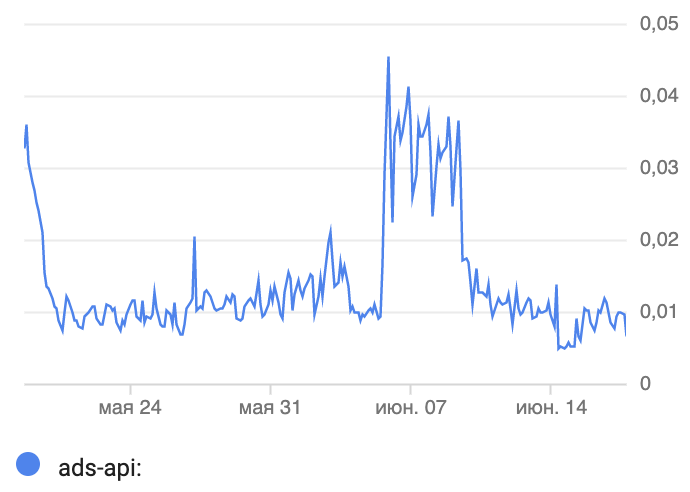
\includegraphics[height=0.2\paperheight]{cpu}
\centering
\label{fig:cpu}
\end{figure}

Ось ординат на графике \ref{fig:cpu} выражена в Millicores  — метрика Kubernetes, которая используется для измерения загрузки процессора (ядро процессора, разделенное на 1000 единиц). Исходя из данных графика видно, что процессор слабо задействован в операциях совершаемых рекламным сервером. 

\begin{figure}[!h]
\caption{Использование RAM репликами рекламного сервера}
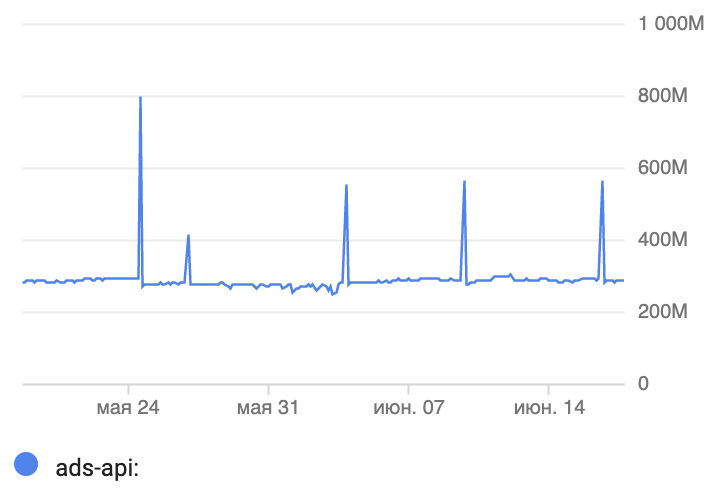
\includegraphics[height=0.2\paperheight]{ram}
\centering
\label{fig:ram}
\end{figure}
График \ref{fig:ram} показывает, что каждая реплика использует порядка 150 Мб RAM в среднем. Пиковые значения на графике обусловены периодическим обновлением образа из репозитория Google Container Registry.


% \section{Нагрузочное тестирование}

% количественные параметры (количество показов, кликов в секунду / сутки, максимальное количество ошибок за сутки / месяц)
% время ответа на 95 процентиле (P95) не более 200 мс


\chapterconclusion

В ходе третьей главы подробно рассмотрен принцип работы моделей: разбиение моделей на сущности, выбранные для их хранения базы данных. Приведено обоснование выбора той или иной базы данных в каждом конкретном случае. Описаны реализации процессов обновления, кэширования рекламных объявлений и обновления категорий интереса пользователей. Приведено описание методов API и контроллеров, обрабатывающих поступающие запросы. Подробно рассмотрен процесс развертывания рекламного сервера в различных окружениях.



%% Макрос для заключения. Совместим со старым стилевиком.
\startconclusionpage

В ходе проделанной работы достигнута поставленная цель и выполнены все необходимые для этого подзадачи:
\begin{itemize}
\item разработан контракт клиент-серверного взаимодействия;
\item разработана архитектура серверного приложения;
\item разработан модуль для создания и обновления рекламных объявлений на основе товаров Amazon;
\item разработан механизм получения списка объявлений с сохранением консистентности;
\item разработаны алгоритмы работы 4-x стратегий таргетинга объявлений;
\item разработана система трекинга просмотров и переходов по объявлениям с возможностью просмотра статистики.
\end{itemize}

Рекламный сервер в виде микросервиса успешно развернут в production-окружении и используется клиентами приложения Fulldive Browser на платформах iOS и Android. Результаты работы рекламного сервера в виде изображений доступны в приложении \ref{sec:app:screenshots}.

В случае успешных договоренностей с компанией Amazon по поводу предоставления возможности отслеживать совершаемые пользователями покупки, станет возможным оптимизировать таргетинг по показателю CPA, что должно увеличить число конверсий.

Дальнейшие разработки и улучшения направлены на:
\begin{itemize}
\item добавление стратегий на основе контекстного таргетинга и улучшение качества работы таргетинга объявлений в целом;
\item улучшение алгоритма фильтрации наиболее привлекательных товаров для целевой аудитории приложений компании;
\item расширение списка поддерживаемых площадок с товарами: Ebay, AliExpress, Wildberries и другие;
\item разработку необходимого функционала для привлечения сторонних рекламодателей;
\item оптимизацию количества и качества рекламного инвентаря в приложениях компании.
\end{itemize}

\printmainbibliography

%% После этой команды chapter будет генерировать приложения, нумерованные русскими буквами.

\appendix

\chapter{Реклама в приложении Fulldive Browser}\label{sec:app:screenshots}

\begin{figure}[h]
\caption{Пример объявления в основной ленте новостей}

\includegraphics[height=0.28\paperheight]{ad-in-feed1}
\centering
\end{figure}

\begin{figure}[h]
\caption{Пример объявления в ленте обсуждаемых новостей}

\includegraphics[height=0.29\paperheight]{ad-in-feed2}
\centering
\end{figure}

\begin{figure}[h]
\caption{Пример списка рекламных объявлений на Android}
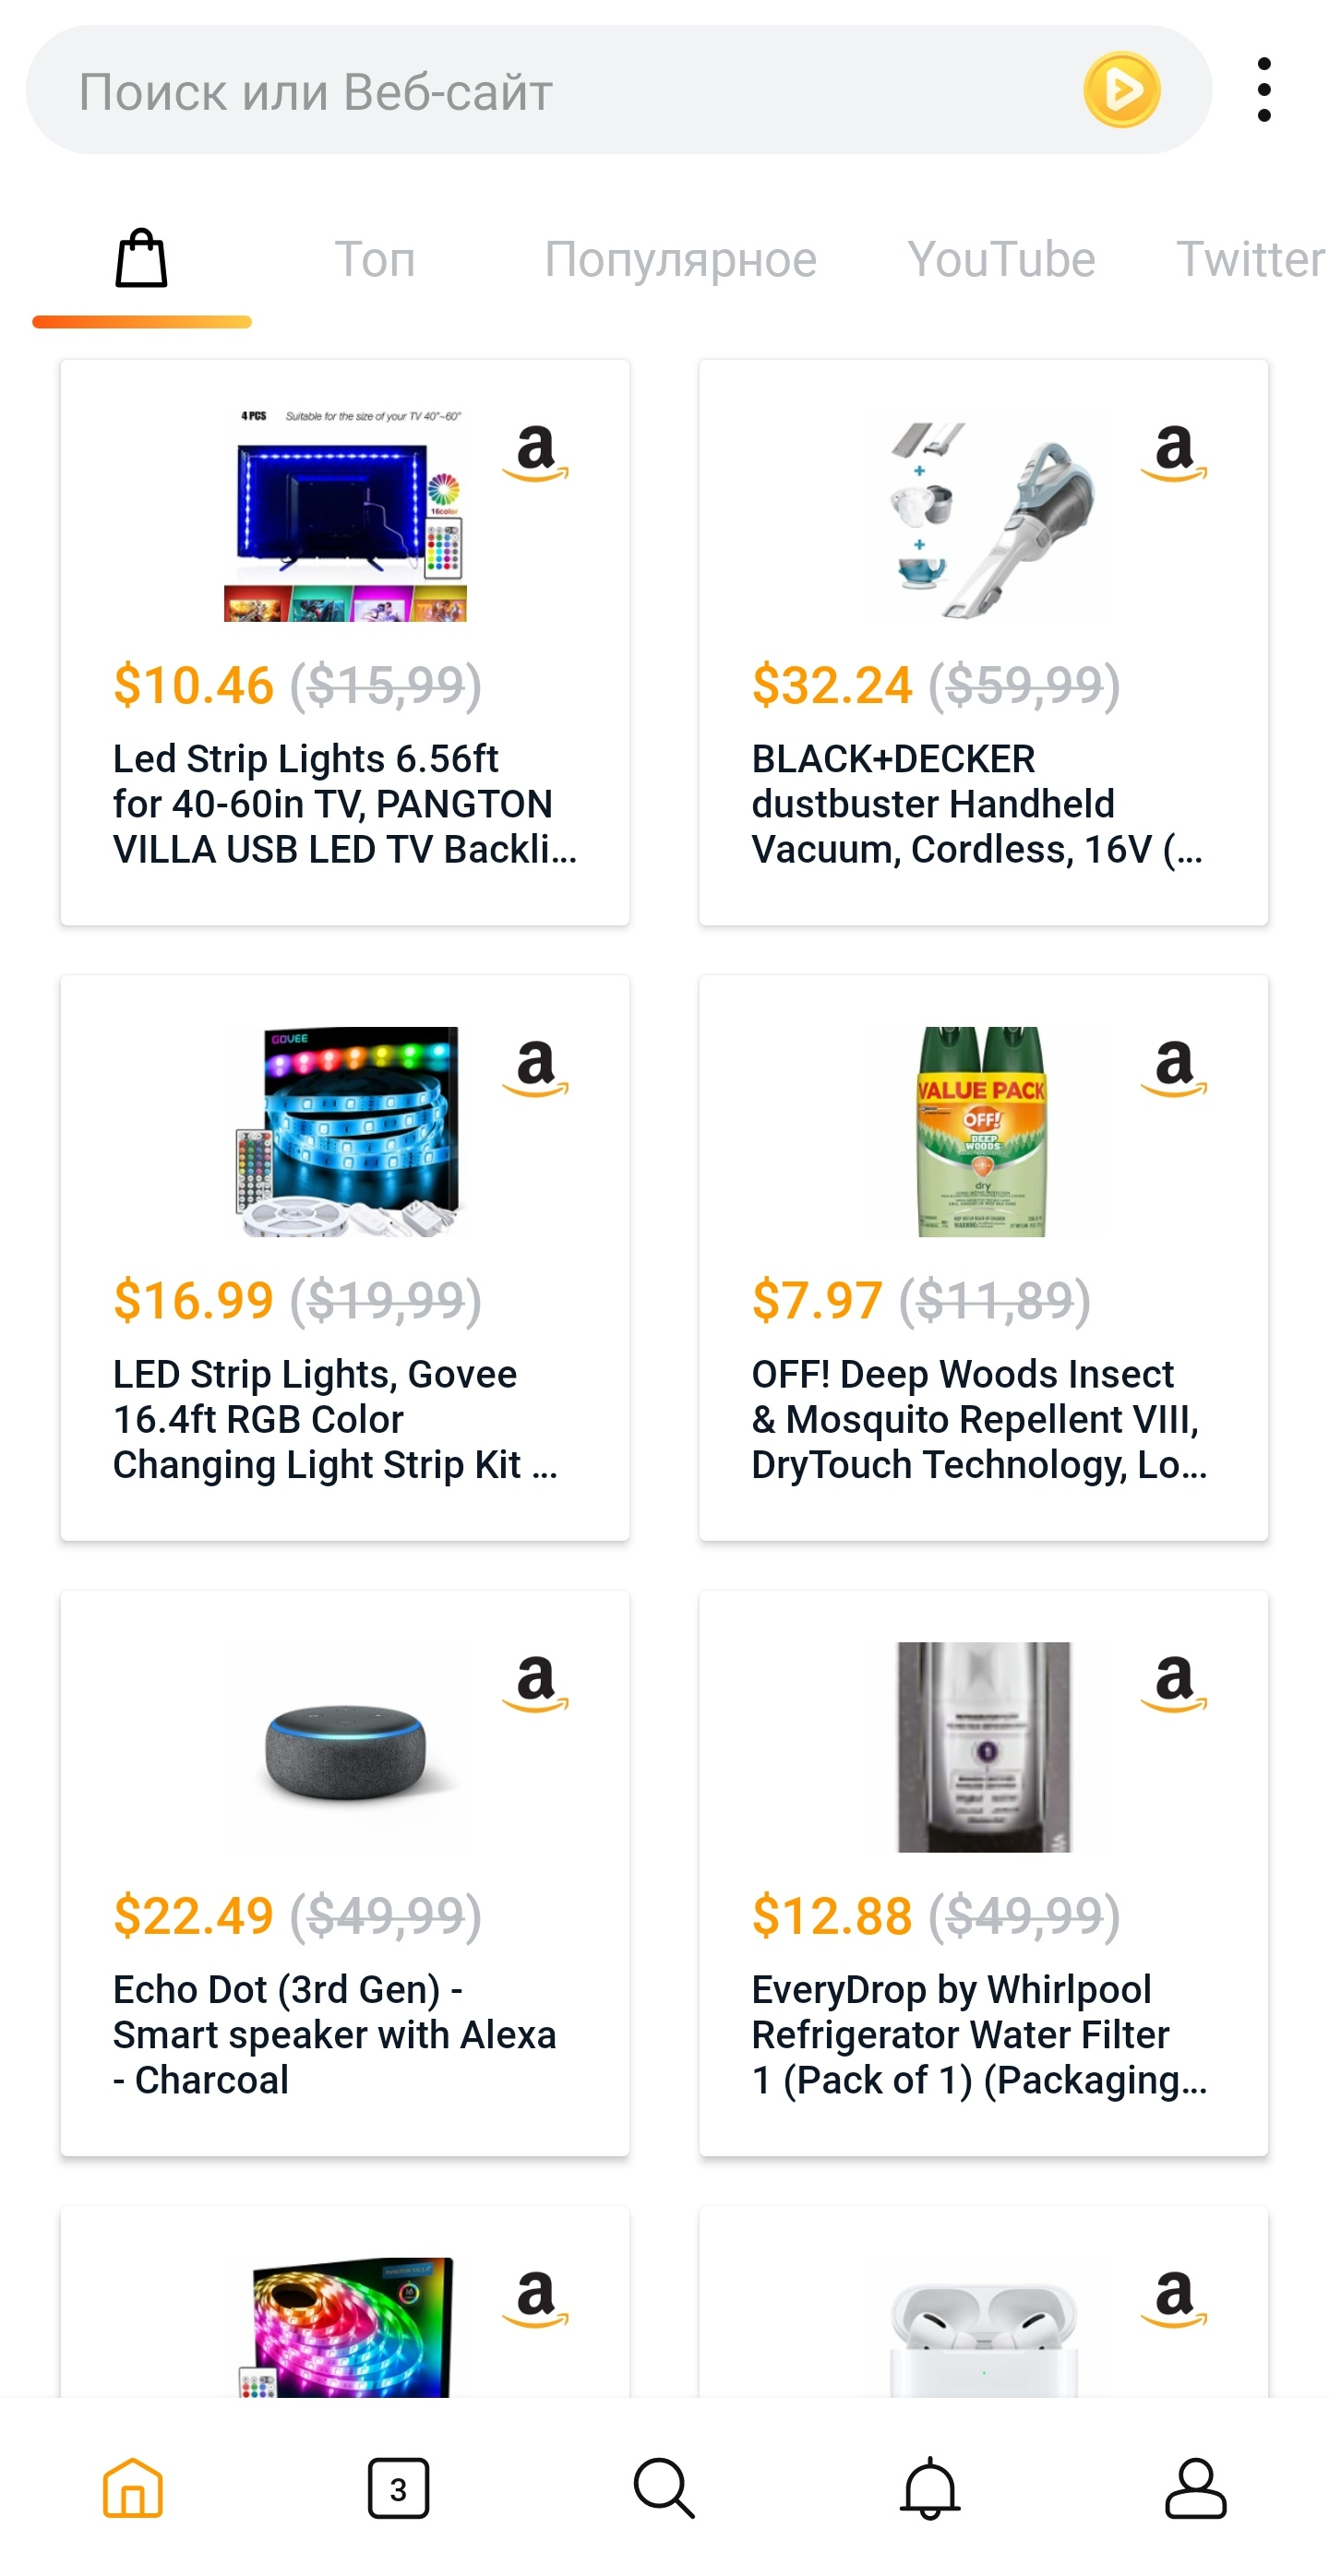
\includegraphics[height=0.35\paperheight]{products-feed-android}
\centering
\end{figure}

\begin{figure}[h]
\caption{Пример списка рекламных объявлений на iOS}
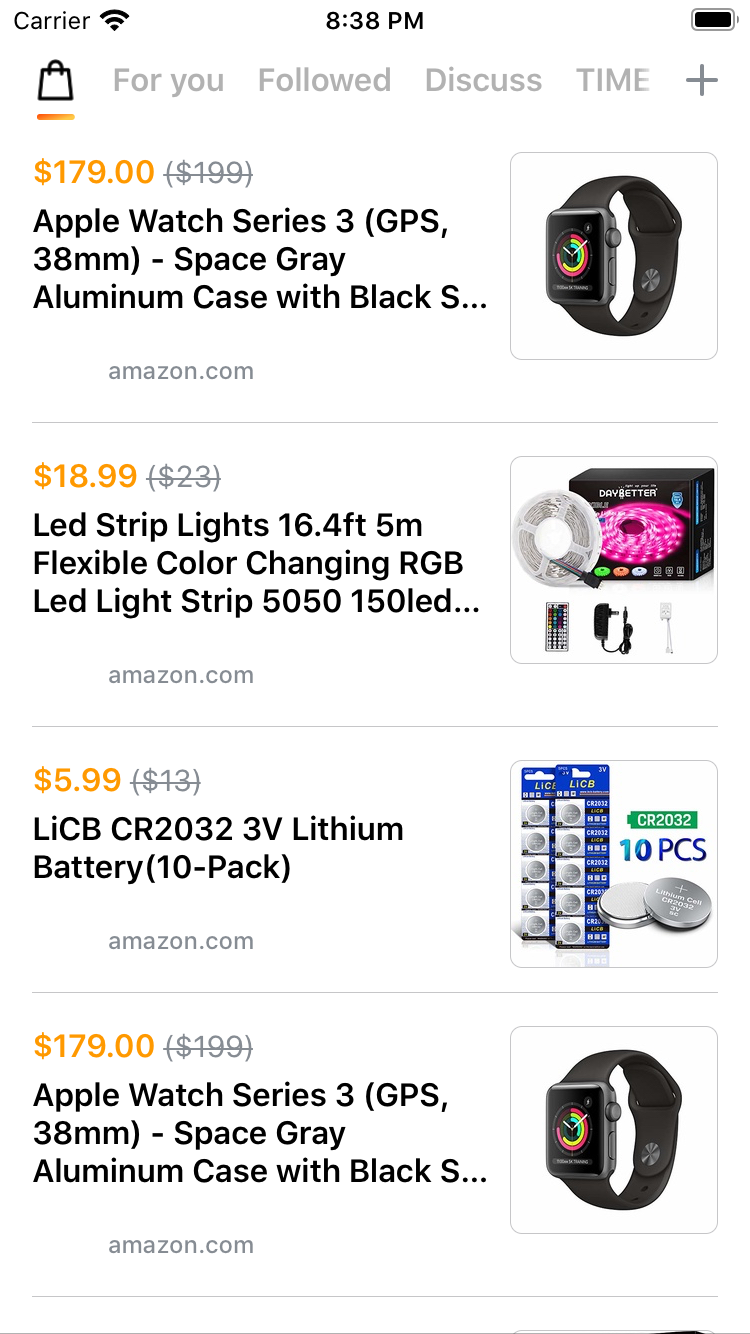
\includegraphics[height=0.35\paperheight]{products-feed-ios}
\centering
\end{figure}

\chapter{Категории товаров на Amazon}\label{sec:app:categories}

\begin{lstlisting}[style=ES6, caption={Список допустимых категорий товаров на Amazon}]
const AMAZON_CATEGORIES = [
    'AmazonVideo',
    'Apparel',
    'Appliances',
    'ArtsAndCrafts',
    'Automotive',
    'Baby',
    'Beauty',
    'Books',
    'Classical',
    'Collectibles',
    'Computers',
    'DigitalMusic',
    'DigitalEducationalResources',
    'Electronics',
    'EverythingElse',
    'Fashion',
    'FashionBaby',
    'FashionBoys',
    'FashionGirls',
    'FashionMen',
    'FashionWomen',
    'GardenAndOutdoor',
    'GiftCards',
    'GroceryAndGourmetFood',
    'Handmade',
    'HealthPersonalCare',
    'HomeAndKitchen',
    'Industrial',
    'Jewelry',
    'KindleStore',
    'LocalServices',
    'Luggage',
    'LuxuryBeauty',
    'Magazines',
    'MobileAndAccessories',
    'MobileApps',
    'MoviesAndTV',
    'Music',
    'MusicalInstruments',
    'OfficeProducts',
    'PetSupplies',
    'Photo',
    'Shoes',
    'Software',
    'SportsAndOutdoors',
    'ToolsAndHomeImprovement',
    'ToysAndGames',
    'VHS',
    'VideoGames',
    'Watches'
]
\end{lstlisting}

\end{document}